% SPDX-License-Identifier: Apache-2.0 OR MIND-UCAL-1.0
% © James Ross Ω FLYING•ROBOTS <https://github.com/flyingrobots>
% Options for packages loaded elsewhere
\PassOptionsToPackage{unicode}{hyperref}
\PassOptionsToPackage{hyphens}{url}
\documentclass[
  11pt,
]{book}
\usepackage{xcolor}
\usepackage[margin=0.75in,letterpaper]{geometry}

\usepackage{graphicx}
\usepackage[export]{adjustbox}
\usepackage{tcolorbox}
\tcbuselibrary{breakable,skins}

% Page layout - small margins
\usepackage[margin=0.75in,letterpaper]{geometry}

% Make code blocks smaller to fit
\usepackage{fvextra}
\DefineVerbatimEnvironment{Highlighting}{Verbatim}{
    commandchars=\\\{\},
    fontsize=\small,
    breaklines=true,
    breakanywhere=true
}

% Define the Claude commentary box style - RED OUTLINE + RED TEXT
\newtcolorbox{claudecommentary}{
    enhanced,
    breakable,
    colback=red!5,
    colframe=red!75!black,
    coltext=red!70!black,
    boxrule=3pt,
    arc=5pt,
    left=12pt,
    right=12pt,
    top=12pt,
    bottom=12pt,
    before skip=15pt,
    after skip=15pt,
    fontupper=\color{red!70!black},
    fonttitle=\bfseries\Large\color{red!75!black},
    title={\raisebox{-0.1em}{\Large$\blacktriangleright$} Claude's Commentary},
    attach boxed title to top left={yshift=-4mm,xshift=10mm},
    boxed title style={
        colback=white,
        colframe=red!75!black,
        boxrule=2pt,
        arc=3pt
    }
}
\usepackage{amsmath,amssymb}
\setcounter{secnumdepth}{-\maxdimen} % remove section numbering
\usepackage{iftex}
\ifPDFTeX
  \usepackage[T1]{fontenc}
  \usepackage[utf8]{inputenc}
  \usepackage{textcomp} % provide euro and other symbols
\else % if luatex or xetex
  \usepackage{unicode-math} % this also loads fontspec
  \defaultfontfeatures{Scale=MatchLowercase}
  \defaultfontfeatures[\rmfamily]{Ligatures=TeX,Scale=1}
\fi
\usepackage{lmodern}
\ifPDFTeX\else
  % xetex/luatex font selection
\fi
% Use upquote if available, for straight quotes in verbatim environments
\IfFileExists{upquote.sty}{\usepackage{upquote}}{}
\IfFileExists{microtype.sty}{% use microtype if available
  \usepackage[]{microtype}
  \UseMicrotypeSet[protrusion]{basicmath} % disable protrusion for tt fonts
}{}
\makeatletter
\@ifundefined{KOMAClassName}{% if non-KOMA class
  \IfFileExists{parskip.sty}{%
    \usepackage{parskip}
  }{% else
    \setlength{\parindent}{0pt}
    \setlength{\parskip}{6pt plus 2pt minus 1pt}}
}{% if KOMA class
  \KOMAoptions{parskip=half}}
\makeatother
\usepackage{color}
\usepackage{fancyvrb}
\newcommand{\VerbBar}{|}
\newcommand{\VERB}{\Verb[commandchars=\\\{\}]}
\DefineVerbatimEnvironment{Highlighting}{Verbatim}{commandchars=\\\{\}}
% Add ',fontsize=\small' for more characters per line
\newenvironment{Shaded}{}{}
\newcommand{\AlertTok}[1]{\textcolor[rgb]{1.00,0.00,0.00}{\textbf{#1}}}
\newcommand{\AnnotationTok}[1]{\textcolor[rgb]{0.38,0.63,0.69}{\textbf{\textit{#1}}}}
\newcommand{\AttributeTok}[1]{\textcolor[rgb]{0.49,0.56,0.16}{#1}}
\newcommand{\BaseNTok}[1]{\textcolor[rgb]{0.25,0.63,0.44}{#1}}
\newcommand{\BuiltInTok}[1]{\textcolor[rgb]{0.00,0.50,0.00}{#1}}
\newcommand{\CharTok}[1]{\textcolor[rgb]{0.25,0.44,0.63}{#1}}
\newcommand{\CommentTok}[1]{\textcolor[rgb]{0.38,0.63,0.69}{\textit{#1}}}
\newcommand{\CommentVarTok}[1]{\textcolor[rgb]{0.38,0.63,0.69}{\textbf{\textit{#1}}}}
\newcommand{\ConstantTok}[1]{\textcolor[rgb]{0.53,0.00,0.00}{#1}}
\newcommand{\ControlFlowTok}[1]{\textcolor[rgb]{0.00,0.44,0.13}{\textbf{#1}}}
\newcommand{\DataTypeTok}[1]{\textcolor[rgb]{0.56,0.13,0.00}{#1}}
\newcommand{\DecValTok}[1]{\textcolor[rgb]{0.25,0.63,0.44}{#1}}
\newcommand{\DocumentationTok}[1]{\textcolor[rgb]{0.73,0.13,0.13}{\textit{#1}}}
\newcommand{\ErrorTok}[1]{\textcolor[rgb]{1.00,0.00,0.00}{\textbf{#1}}}
\newcommand{\ExtensionTok}[1]{#1}
\newcommand{\FloatTok}[1]{\textcolor[rgb]{0.25,0.63,0.44}{#1}}
\newcommand{\FunctionTok}[1]{\textcolor[rgb]{0.02,0.16,0.49}{#1}}
\newcommand{\ImportTok}[1]{\textcolor[rgb]{0.00,0.50,0.00}{\textbf{#1}}}
\newcommand{\InformationTok}[1]{\textcolor[rgb]{0.38,0.63,0.69}{\textbf{\textit{#1}}}}
\newcommand{\KeywordTok}[1]{\textcolor[rgb]{0.00,0.44,0.13}{\textbf{#1}}}
\newcommand{\NormalTok}[1]{#1}
\newcommand{\OperatorTok}[1]{\textcolor[rgb]{0.40,0.40,0.40}{#1}}
\newcommand{\OtherTok}[1]{\textcolor[rgb]{0.00,0.44,0.13}{#1}}
\newcommand{\PreprocessorTok}[1]{\textcolor[rgb]{0.74,0.48,0.00}{#1}}
\newcommand{\RegionMarkerTok}[1]{#1}
\newcommand{\SpecialCharTok}[1]{\textcolor[rgb]{0.25,0.44,0.63}{#1}}
\newcommand{\SpecialStringTok}[1]{\textcolor[rgb]{0.73,0.40,0.53}{#1}}
\newcommand{\StringTok}[1]{\textcolor[rgb]{0.25,0.44,0.63}{#1}}
\newcommand{\VariableTok}[1]{\textcolor[rgb]{0.10,0.09,0.49}{#1}}
\newcommand{\VerbatimStringTok}[1]{\textcolor[rgb]{0.25,0.44,0.63}{#1}}
\newcommand{\WarningTok}[1]{\textcolor[rgb]{0.38,0.63,0.69}{\textbf{\textit{#1}}}}
\usepackage{longtable,booktabs,array}
\newcounter{none} % for unnumbered tables
\usepackage{calc} % for calculating minipage widths
% Correct order of tables after \paragraph or \subparagraph
\usepackage{etoolbox}
\makeatletter
\patchcmd\longtable{\par}{\if@noskipsec\mbox{}\fi\par}{}{}
\makeatother
% Allow footnotes in longtable head/foot
\IfFileExists{footnotehyper.sty}{\usepackage{footnotehyper}}{\usepackage{footnote}}
\makesavenoteenv{longtable}
\usepackage{graphicx}
\makeatletter
\newsavebox\pandoc@box
\newcommand*\pandocbounded[1]{% scales image to fit in text height/width
  \sbox\pandoc@box{#1}%
  \Gscale@div\@tempa{\textheight}{\dimexpr\ht\pandoc@box+\dp\pandoc@box\relax}%
  \Gscale@div\@tempb{\linewidth}{\wd\pandoc@box}%
  \ifdim\@tempb\p@<\@tempa\p@\let\@tempa\@tempb\fi% select the smaller of both
  \ifdim\@tempa\p@<\p@\scalebox{\@tempa}{\usebox\pandoc@box}%
  \else\usebox{\pandoc@box}%
  \fi%
}
% Set default figure placement to htbp
\def\fps@figure{htbp}
\makeatother
\setlength{\emergencystretch}{3em} % prevent overfull lines
\providecommand{\tightlist}{%
  \setlength{\itemsep}{0pt}\setlength{\parskip}{0pt}}
\usepackage{bookmark}
\IfFileExists{xurl.sty}{\usepackage{xurl}}{} % add URL line breaks if available
\urlstyle{same}
\hypersetup{
  hidelinks,
  pdfcreator={LaTeX via pandoc}}

\author{}
\date{}

\begin{document}
\frontmatter

\mainmatter
\chapter{What Makes Echo Tick?}\label{what-makes-echo-tick}

\begin{quote}
\textbf{Your Tour Guide}: Claude (Opus 4.5)

Welcome! I've been asked to give you a personal tour through Echo's
internals. This isn't just documentation---I'll share what I find
elegant, surprising, and occasionally baffling about this codebase. When
you see a red-outlined box, that's me stepping out of ``narrator mode''
to give you my unfiltered take.

\textbf{Reading Time}: \textasciitilde45 minutes for complete
understanding.
\end{quote}

\begin{center}\rule{0.5\linewidth}{0.5pt}\end{center}

\section{Table of Contents}\label{table-of-contents}

\begin{enumerate}
\def\labelenumi{\arabic{enumi}.}
\tightlist
\item
  \hyperref[1-philosophy-why-echo-exists]{Philosophy: Why Echo Exists}
\item
  \hyperref[2-the-big-picture-architecture-overview]{The Big Picture:
  Architecture Overview}
\item
  \hyperref[3-core-concepts-the-warp-graph]{Core Concepts: The WARP
  Graph}
\item
  \hyperref[4-the-engine-heart-of-echo]{The Engine: Heart of Echo}
\item
  \hyperref[5-the-tick-pipeline-where-everything-happens]{The Tick
  Pipeline: Where Everything Happens}
\item
  \hyperref[6-parallel-execution-boaw-bag-of-autonomous-workers]{Parallel
  Execution: BOAW (Bag of Autonomous Workers)}
\item
  \hyperref[7-storage--hashing-content-addressed-truth]{Storage \&
  Hashing: Content-Addressed Truth}
\item
  \hyperref[8-worked-example-tracing-a-link-click]{Worked Example:
  Tracing a Link Click}
\item
  \hyperref[9-the-viewer-observing-echo]{The Viewer: Observing Echo}
\item
  \hyperref[10-glossary]{Glossary}
\end{enumerate}

\begin{center}\rule{0.5\linewidth}{0.5pt}\end{center}

\section{1. Philosophy: Why Echo
Exists}\label{philosophy-why-echo-exists}

\subsection{1.1 The Problem}\label{the-problem}

Traditional game engines and simulations treat state as \textbf{mutable
objects}. This creates fundamental problems:

\begin{itemize}
\tightlist
\item
  \textbf{Replay is hard}: You can't just ``rewind'' because state
  changes are scattered and untracked.
\item
  \textbf{Synchronization is fragile}: Two machines running the same
  logic may diverge due to floating-point differences, thread timing, or
  iteration order.
\item
  \textbf{Debugging is a nightmare}: ``It worked on my machine'' is the
  symptom of non-determinism.
\item
  \textbf{Branching is impossible}: You can't easily ask ``what if?''
  without copying everything.
\end{itemize}

\begin{claudecommentary}
**Claude's Take**: This list of problems isn't theoretical. I've seen countless debugging sessions where the root cause was "HashMap iteration order changed between runs." Echo's designers clearly got burned by non-determinism at some point and decided: *never again*.

What strikes me most is the last point—"branching is impossible." Most engines don't even *try* to support branching because it seems like a feature for version control, not runtime systems. Echo treats it as a first-class concern. That's unusual and, I think, genuinely forward-thinking.
\end{claudecommentary}

\subsection{1.2 Echo's Answer}\label{echos-answer}

Echo treats \textbf{state as a typed graph} and \textbf{all changes as
rewrites}. Each ``tick'' of the engine:

\begin{enumerate}
\def\labelenumi{\arabic{enumi}.}
\tightlist
\item
  Proposes a set of rewrites
\item
  Executes them in \textbf{deterministic order}
\item
  Emits \textbf{cryptographic hashes} of the resulting state
\end{enumerate}

This means: - \textbf{Same inputs → Same outputs} (always, on any
machine) - \textbf{State is verifiable} (hashes prove correctness) -
\textbf{Replay is trivial} (patches are prescriptive) -
\textbf{Branching is free} (copy-on-write snapshots)

\subsection{1.3 Core Design Principles}\label{core-design-principles}

\begin{verbatim}
┌─────────────────────────────────────────────────────────────────┐
│                    ECHO'S THREE PILLARS                          │
├─────────────────────────────────────────────────────────────────┤
│                                                                  │
│  ┌─────────────────┐  ┌─────────────────┐  ┌─────────────────┐  │
│  │   DETERMINISM   │  │   PROVENANCE    │  │    TOOLING      │  │
│  │     FIRST       │  │   YOU CAN       │  │   AS FIRST      │  │
│  │                 │  │     TRUST       │  │     CLASS       │  │
│  ├─────────────────┤  ├─────────────────┤  ├─────────────────┤  │
│  │ Same inputs     │  │ Snapshots are   │  │ Graphs stream   │  │
│  │ always produce  │  │ content-        │  │ over canonical  │  │
│  │ same hashes     │  │ addressed       │  │ wire protocol   │  │
│  └─────────────────┘  └─────────────────┘  └─────────────────┘  │
│                                                                  │
└─────────────────────────────────────────────────────────────────┘
\end{verbatim}

\begin{claudecommentary}
**Claude's Take**: "Tooling as first-class" is the sleeper here. Most engines treat debugging tools, replay systems, and visualization as afterthoughts—bolted on after the core is done. Echo inverts this: the wire protocol, the hash scheme, and the diff format were designed *so that tools could exist*.

I've read a lot of engine architectures. This level of intentionality about tooling is rare. It's also why Echo can have a separate `warp-viewer` crate that just... works, instead of requiring heroic reverse-engineering.
\end{claudecommentary}

\begin{center}\rule{0.5\linewidth}{0.5pt}\end{center}

\section{2. The Big Picture: Architecture
Overview}\label{the-big-picture-architecture-overview}

\subsection{2.1 System Layers}\label{system-layers}

Echo is organized into distinct layers, each with a specific
responsibility:

\begin{figure}
\centering
\pandocbounded{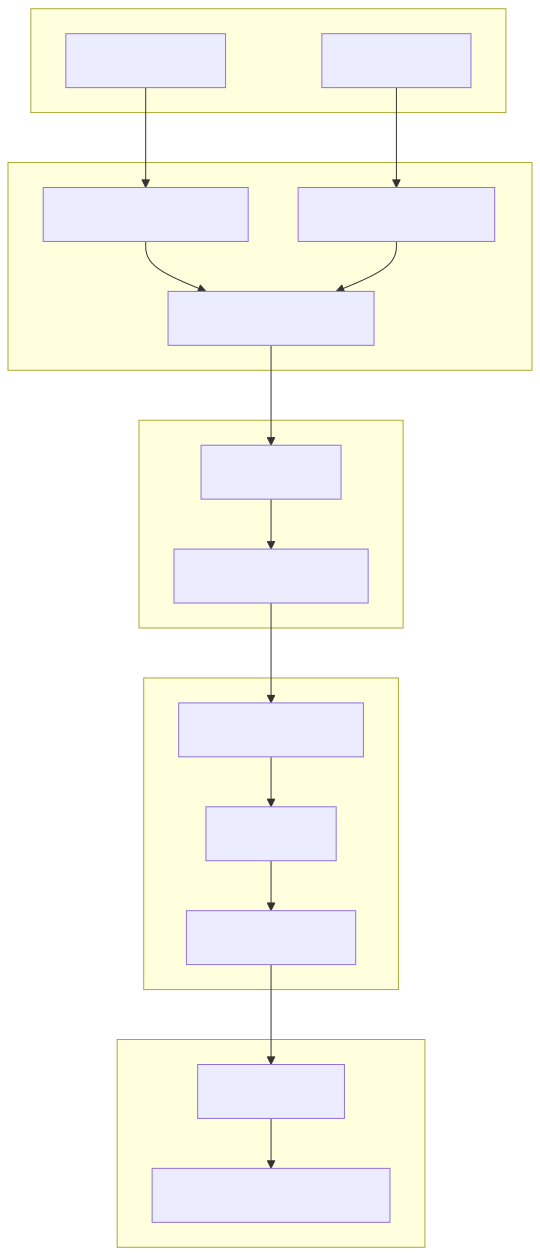
\includegraphics[keepaspectratio,alt={Diagram 1}]{diagrams/tour-01.pdf}}
\caption{Diagram 1}
\end{figure}

\begin{claudecommentary}
**Claude's Take**: This is a *clean* layer cake. Each layer only talks to its neighbors. No "Layer 5 reaching down to Layer 1 for performance reasons." That discipline is hard to maintain, and I respect it.

The `WSC Format` at Layer 2 caught my eye. It's Echo's custom columnar storage format—and before you ask "why not just use Arrow or Parquet?"—I'll spoil it: WSC is designed for mmap-friendly, zero-copy reads where every row is 8-byte aligned and you can binary-search directly into the file. It's specialized for *exactly this use case*. Sometimes NIH syndrome is justified.
\end{claudecommentary}

\subsection{2.2 Crate Map}\label{crate-map}

{\def\LTcaptype{none} % do not increment counter
\begin{longtable}[]{@{}ll@{}}
\toprule\noalign{}
Crate & Purpose \\
\midrule\noalign{}
\endhead
\bottomrule\noalign{}
\endlastfoot
\texttt{warp-core} & The deterministic rewrite engine (the ``brain'') \\
\texttt{echo-graph} & Renderable graph types + diff operations \\
\texttt{echo-session-proto} & Wire protocol (canonical CBOR framing) \\
\texttt{echo-session-service} & Headless Unix-socket hub for tools \\
\texttt{echo-session-client} & Client helpers for connecting to the
hub \\
\texttt{warp-viewer} & Native WGPU viewer for visualizing graphs \\
\end{longtable}
}

\subsection{2.3 Data Flow Overview}\label{data-flow-overview}

\begin{figure}
\centering
\pandocbounded{\includegraphics[keepaspectratio,alt={Diagram 2}]{diagrams/tour-02.pdf}}
\caption{Diagram 2}
\end{figure}

\begin{claudecommentary}
**Claude's Take**: Notice how the Engine talks to itself multiple times before touching the Store? That's the commit protocol at work. The Engine is *paranoid* about mutations—it queues up intentions, validates them, and only then touches state. If you're used to "just mutate it directly" game engines, this will feel ceremonial. The ceremony is the point.
\end{claudecommentary}

\begin{center}\rule{0.5\linewidth}{0.5pt}\end{center}

\section{3. Core Concepts: The WARP
Graph}\label{core-concepts-the-warp-graph}

\subsection{3.1 What is a WARP Graph?}\label{what-is-a-warp-graph}

A WARP (\textbf{W}orldline \textbf{A}lgebra for \textbf{R}ecursive
\textbf{P}rovenance) graph is Echo's fundamental data structure. It's
not just a graph---it's a graph with \textbf{deterministic semantics}.

\begin{figure}
\centering
\pandocbounded{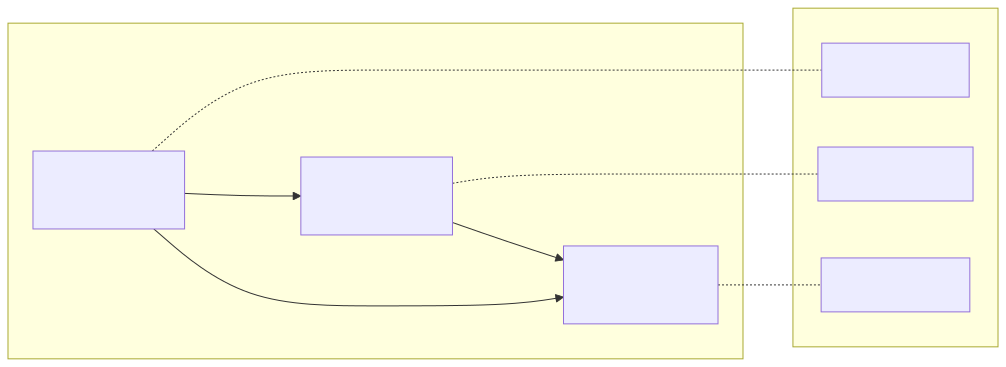
\includegraphics[keepaspectratio,alt={Diagram 3}]{diagrams/tour-03.pdf}}
\caption{Diagram 3}
\end{figure}

\begin{claudecommentary}
**Claude's Take**: The name "WARP" is doing a lot of work here. "Worldline" evokes physics—specifically, the path an object traces through spacetime. In Echo, a node's "worldline" is its history of states across ticks. "Recursive Provenance" means you can always ask "where did this value come from?" and trace it back through the graph's history.

Is the name a bit grandiose for what amounts to "typed graph with audit trail"? Maybe. But I've seen worse acronyms in this industry.
\end{claudecommentary}

\subsection{3.2 Two-Plane Architecture}\label{two-plane-architecture}

Echo separates structure from data via the \textbf{Two-Plane Model}
(ADR-0001):

{\def\LTcaptype{none} % do not increment counter
\begin{longtable}[]{@{}
  >{\raggedright\arraybackslash}p{(\linewidth - 4\tabcolsep) * \real{0.2692}}
  >{\raggedright\arraybackslash}p{(\linewidth - 4\tabcolsep) * \real{0.3846}}
  >{\raggedright\arraybackslash}p{(\linewidth - 4\tabcolsep) * \real{0.3462}}@{}}
\toprule\noalign{}
\begin{minipage}[b]{\linewidth}\raggedright
Plane
\end{minipage} & \begin{minipage}[b]{\linewidth}\raggedright
Contains
\end{minipage} & \begin{minipage}[b]{\linewidth}\raggedright
Purpose
\end{minipage} \\
\midrule\noalign{}
\endhead
\bottomrule\noalign{}
\endlastfoot
\textbf{Skeleton} & Nodes + Edges (structure) & Fast traversal,
deterministic hashing \\
\textbf{Attachment (α)} & Typed payloads & Domain-specific data \\
\end{longtable}
}

\textbf{Why separate them?}

\begin{verbatim}
┌────────────────────────────────────────────────────────────────────┐
│ SKELETON PLANE (Structure)                                          │
│                                                                     │
│   ┌─────┐    edge:link     ┌─────┐                                 │
│   │ N1  │─────────────────▶│ N2  │                                 │
│   └─────┘                   └─────┘                                 │
│      │                         │                                    │
│      │ edge:child              │ edge:ref                          │
│      ▼                         ▼                                    │
│   ┌─────┐◀─────────────────────┘                                   │
│   │ N3  │                                                          │
│   └─────┘                                                          │
│                                                                     │
├────────────────────────────────────────────────────────────────────┤
│ ATTACHMENT PLANE (Payloads)                                         │
│                                                                     │
│   N1.α["title"] = Atom { type: "string", bytes: "Home" }           │
│   N2.α["url"]   = Atom { type: "string", bytes: "/page/b" }        │
│   N3.α["body"]  = Atom { type: "html",   bytes: "<p>...</p>" }     │
│                                                                     │
└────────────────────────────────────────────────────────────────────┘
\end{verbatim}

\textbf{Key insight}: Skeleton rewrites \textbf{never decode
attachments}. This keeps the hot path fast and deterministic.

\begin{claudecommentary}
**Claude's Take**: This is where Echo gets clever. The Skeleton plane only contains node IDs, edge IDs, and type tags—all fixed-size, all byte-comparable. You can compute the entire state hash without ever deserializing a single JSON blob, HTML string, or texture.

The Attachment plane (they call it "α" because of course they do) holds the actual domain data. It participates in hashing but doesn't affect traversal. This separation means you can have a 10MB texture attached to a node and still iterate the graph at full speed.

I've seen similar ideas in ECS architectures, but usually the separation is "components vs. systems." Echo's split is "structure vs. data," which is subtly different and, I think, more principled.
\end{claudecommentary}

\subsection{3.3 Node and Edge Identity}\label{node-and-edge-identity}

Every node and edge has a \textbf{32-byte identifier}:

\begin{Shaded}
\begin{Highlighting}[]
\KeywordTok{pub} \KeywordTok{struct}\NormalTok{ NodeId([}\DataTypeTok{u8}\OperatorTok{;} \DecValTok{32}\NormalTok{])}\OperatorTok{;}  \CommentTok{// Content{-}addressed or assigned}
\KeywordTok{pub} \KeywordTok{struct}\NormalTok{ EdgeId([}\DataTypeTok{u8}\OperatorTok{;} \DecValTok{32}\NormalTok{])}\OperatorTok{;}  \CommentTok{// Unique edge identifier}
\end{Highlighting}
\end{Shaded}

These IDs are: - \textbf{Deterministic}: Same content → same ID (when
content-addressed) - \textbf{Sortable}: Lexicographic ordering enables
deterministic iteration - \textbf{Hashable}: Participate in state root
computation

\subsection{3.4 WarpInstances: Graphs Within
Graphs}\label{warpinstances-graphs-within-graphs}

Echo supports \textbf{descended attachments}---embedding entire graphs
within attachment slots:

\begin{figure}
\centering
\pandocbounded{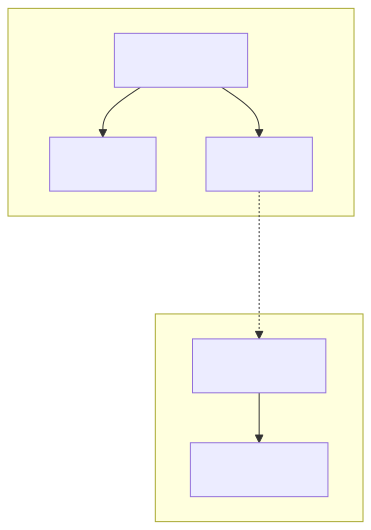
\includegraphics[keepaspectratio,alt={Diagram 4}]{diagrams/tour-04.pdf}}
\caption{Diagram 4}
\end{figure}

This enables ``WARPs all the way down''---recursive composition while
maintaining determinism.

\begin{claudecommentary}
**Claude's Take**: WarpInstances are *wild*. You can have a node whose attachment slot contains... another entire graph. And that graph can have nodes whose attachment slots contain... more graphs. It's turtles, but the turtles are graphs.

Why would you want this? Think of a game with procedurally generated dungeons. Each dungeon could be its own WarpInstance, loaded on demand, with its own tick history and state root. The player character is in the "outer" instance; stepping through a portal descends into the "inner" one.

I don't know if Echo actually uses this feature yet, but the architecture supports it cleanly. That's design for the future without overengineering the present.
\end{claudecommentary}

\begin{center}\rule{0.5\linewidth}{0.5pt}\end{center}

\section{4. The Engine: Heart of Echo}\label{the-engine-heart-of-echo}

\subsection{4.1 The Engine Struct}\label{the-engine-struct}

The \texttt{Engine} is Echo's central orchestrator. Located in
\texttt{crates/warp-core/src/engine\_impl.rs}:

\begin{Shaded}
\begin{Highlighting}[]
\KeywordTok{pub} \KeywordTok{struct}\NormalTok{ Engine }\OperatorTok{\{}
\NormalTok{    state}\OperatorTok{:}\NormalTok{ WarpState}\OperatorTok{,}                           \CommentTok{// Multi{-}instance graph state}
\NormalTok{    rules}\OperatorTok{:}\NormalTok{ HashMap}\OperatorTok{\textless{}}\NormalTok{RuleId}\OperatorTok{,}\NormalTok{ RewriteRule}\OperatorTok{\textgreater{},}        \CommentTok{// Registered rewrite rules}
\NormalTok{    scheduler}\OperatorTok{:}\NormalTok{ DeterministicScheduler}\OperatorTok{,}          \CommentTok{// Deterministic ordering}
\NormalTok{    bus}\OperatorTok{:}\NormalTok{ MaterializationBus}\OperatorTok{,}                    \CommentTok{// Output channels}
\NormalTok{    history}\OperatorTok{:} \DataTypeTok{Vec}\OperatorTok{\textless{}}\NormalTok{(Snapshot}\OperatorTok{,}\NormalTok{ TickReceipt}\OperatorTok{,}\NormalTok{ WarpTickPatchV1)}\OperatorTok{\textgreater{},}
\NormalTok{    tx\_counter}\OperatorTok{:} \DataTypeTok{u64}\OperatorTok{,}                            \CommentTok{// Transaction counter}
\NormalTok{    live\_txs}\OperatorTok{:}\NormalTok{ BTreeSet}\OperatorTok{\textless{}}\NormalTok{TxId}\OperatorTok{\textgreater{},}                   \CommentTok{// Active transactions}
    \CommentTok{// ... more fields}
\OperatorTok{\}}
\end{Highlighting}
\end{Shaded}

\begin{claudecommentary}
**Claude's Take**: A few things jump out here:

1. **`rules: HashMap<RuleId, RewriteRule>`** — Wait, HashMap? Isn't that non-deterministic? It is! But notice: this is for *looking up* rules by ID, not for *iterating*. The iteration order is determined by the `scheduler`, which is explicitly deterministic. The HashMap is fine because rule IDs are stable.

2. **`history: Vec<(Snapshot, TickReceipt, WarpTickPatchV1)>`** — The engine keeps its entire history in memory? That seems expensive. I suspect this is configurable, or there's a garbage collection pass I haven't found yet. For long-running simulations, unbounded history would be a problem.

3. **`BTreeSet<TxId>` for live transactions** — BTreeSet, not HashSet. They're *really* committed to determinism. Even the set of "which transactions are in-flight" is stored in sorted order.
\end{claudecommentary}

\subsection{4.2 Construction}\label{construction}

The engine is built via the \texttt{EngineBuilder}:

\begin{Shaded}
\begin{Highlighting}[]
\KeywordTok{let}\NormalTok{ engine }\OperatorTok{=} \PreprocessorTok{EngineBuilder::}\NormalTok{new(store}\OperatorTok{,}\NormalTok{ root\_node\_id)}
    \OperatorTok{.}\NormalTok{with\_policy\_id(}\DecValTok{1}\NormalTok{)}
    \OperatorTok{.}\NormalTok{with\_telemetry(telemetry)}
    \OperatorTok{.}\NormalTok{build()}\OperatorTok{;}
\end{Highlighting}
\end{Shaded}

\textbf{What happens during construction:}

\begin{figure}
\centering
\pandocbounded{\includegraphics[keepaspectratio,alt={Diagram 5}]{diagrams/tour-05.pdf}}
\caption{Diagram 5}
\end{figure}

\subsection{4.3 Rewrite Rules}\label{rewrite-rules}

Rules are the atoms of change in Echo. Each rule has three functions:

\begin{Shaded}
\begin{Highlighting}[]
\KeywordTok{pub} \KeywordTok{struct}\NormalTok{ RewriteRule }\OperatorTok{\{}
    \KeywordTok{pub}\NormalTok{ name}\OperatorTok{:} \DataTypeTok{String}\OperatorTok{,}
    \KeywordTok{pub}\NormalTok{ matcher}\OperatorTok{:}\NormalTok{ MatchFn}\OperatorTok{,}      \CommentTok{// Does this rule apply?}
    \KeywordTok{pub}\NormalTok{ executor}\OperatorTok{:}\NormalTok{ ExecuteFn}\OperatorTok{,}    \CommentTok{// What changes to make}
    \KeywordTok{pub}\NormalTok{ footprint}\OperatorTok{:}\NormalTok{ FootprintFn}\OperatorTok{,} \CommentTok{// What resources are touched}
    \KeywordTok{pub}\NormalTok{ policy}\OperatorTok{:}\NormalTok{ ConflictPolicy}\OperatorTok{,} \CommentTok{// What to do on conflict}
\OperatorTok{\}}

\CommentTok{// Function signatures (Phase 5 BOAW model):}
\KeywordTok{type}\NormalTok{ MatchFn    }\OperatorTok{=} \KeywordTok{fn}\NormalTok{(GraphView}\OperatorTok{,} \OperatorTok{\&}\NormalTok{NodeId) }\OperatorTok{{-}\textgreater{}} \DataTypeTok{bool}\OperatorTok{;}
\KeywordTok{type}\NormalTok{ ExecuteFn  }\OperatorTok{=} \KeywordTok{fn}\NormalTok{(GraphView}\OperatorTok{,} \OperatorTok{\&}\NormalTok{NodeId}\OperatorTok{,} \OperatorTok{\&}\KeywordTok{mut}\NormalTok{ TickDelta)}\OperatorTok{;}
\KeywordTok{type}\NormalTok{ FootprintFn }\OperatorTok{=} \KeywordTok{fn}\NormalTok{(GraphView}\OperatorTok{,} \OperatorTok{\&}\NormalTok{NodeId) }\OperatorTok{{-}\textgreater{}}\NormalTok{ Footprint}\OperatorTok{;}
\end{Highlighting}
\end{Shaded}

\textbf{Critical constraint}: Executors receive a \textbf{read-only}
\texttt{GraphView} and emit changes to a \texttt{TickDelta}. They
\textbf{never} mutate the graph directly.

\begin{claudecommentary}
**Claude's Take**: The `FootprintFn` is the secret sauce. Before executing a rule, Echo calls this function to ask: "What nodes, edges, and attachments will you touch?" The footprint is a *conservative estimate*—you must declare everything you *might* read or write.

This enables Echo's parallel execution model. If two rules have non-overlapping footprints, they can execute in parallel, in any order, and the result is guaranteed identical. If footprints overlap, they're sequenced deterministically.

The burden on the rule author is significant: you must declare your footprint accurately, or you'll get either conflicts (declared overlap when there was none) or silent bugs (undeclared overlap that corrupts state). This is a sharp edge in the API.
\end{claudecommentary}

\subsection{4.4 GraphView: Read-Only
Access}\label{graphview-read-only-access}

The \texttt{GraphView} enforces BOAW's immutability contract:

\begin{Shaded}
\begin{Highlighting}[]
\KeywordTok{pub} \KeywordTok{struct}\NormalTok{ GraphView}\OperatorTok{\textless{}}\OtherTok{\textquotesingle{}a}\OperatorTok{\textgreater{}} \OperatorTok{\{}
\NormalTok{    store}\OperatorTok{:} \OperatorTok{\&}\OtherTok{\textquotesingle{}a}\NormalTok{ GraphStore}\OperatorTok{,}
\NormalTok{    warp\_id}\OperatorTok{:}\NormalTok{ WarpId}\OperatorTok{,}
\OperatorTok{\}}

\KeywordTok{impl}\OperatorTok{\textless{}}\OtherTok{\textquotesingle{}a}\OperatorTok{\textgreater{}}\NormalTok{ GraphView}\OperatorTok{\textless{}}\OtherTok{\textquotesingle{}a}\OperatorTok{\textgreater{}} \OperatorTok{\{}
    \KeywordTok{pub} \KeywordTok{fn}\NormalTok{ node(}\OperatorTok{\&}\KeywordTok{self}\OperatorTok{,}\NormalTok{ id}\OperatorTok{:} \OperatorTok{\&}\NormalTok{NodeId) }\OperatorTok{{-}\textgreater{}} \DataTypeTok{Option}\OperatorTok{\textless{}\&}\NormalTok{NodeRecord}\OperatorTok{\textgreater{};}
    \KeywordTok{pub} \KeywordTok{fn}\NormalTok{ edges\_from(}\OperatorTok{\&}\KeywordTok{self}\OperatorTok{,}\NormalTok{ id}\OperatorTok{:} \OperatorTok{\&}\NormalTok{NodeId) }\OperatorTok{{-}\textgreater{}} \KeywordTok{impl} \BuiltInTok{Iterator}\OperatorTok{\textless{}}\NormalTok{Item }\OperatorTok{=} \OperatorTok{\&}\NormalTok{EdgeRecord}\OperatorTok{\textgreater{};}
    \KeywordTok{pub} \KeywordTok{fn}\NormalTok{ node\_attachment(}\OperatorTok{\&}\KeywordTok{self}\OperatorTok{,}\NormalTok{ id}\OperatorTok{:} \OperatorTok{\&}\NormalTok{NodeId}\OperatorTok{,}\NormalTok{ key}\OperatorTok{:} \OperatorTok{\&}\DataTypeTok{str}\NormalTok{) }\OperatorTok{{-}\textgreater{}} \DataTypeTok{Option}\OperatorTok{\textless{}\&}\NormalTok{AttachmentValue}\OperatorTok{\textgreater{};}
    \CommentTok{// ... read{-}only methods only}
\OperatorTok{\}}
\end{Highlighting}
\end{Shaded}

\textbf{No \texttt{DerefMut}, no
\texttt{AsRef\textless{}GraphStore\textgreater{}}, no interior
mutability.} This is enforced at the type level.

\begin{claudecommentary}
**Claude's Take**: I went looking for escape hatches here. `RefCell`? No. `UnsafeCell`? No. `Arc<Mutex<...>>`? No. The `GraphView` is genuinely immutable by construction.

This is Rust at its best: the borrow checker prevents you from shooting yourself in the foot. In C++, you'd need discipline and code review to enforce "executors don't mutate the graph." In Rust, it's just... not possible. The types don't allow it.
\end{claudecommentary}

\begin{center}\rule{0.5\linewidth}{0.5pt}\end{center}

\section{5. The Tick Pipeline: Where Everything
Happens}\label{the-tick-pipeline-where-everything-happens}

\subsection{5.1 Overview}\label{overview}

A ``tick'' is one complete cycle of the engine. It has five phases:

\begin{figure}
\centering
\pandocbounded{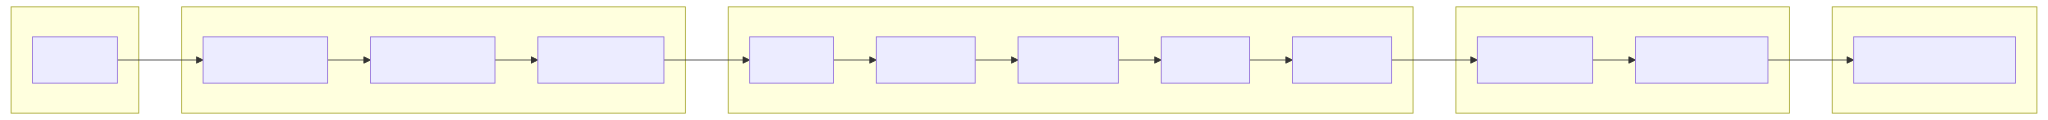
\includegraphics[keepaspectratio,alt={Diagram 6}]{diagrams/tour-06.pdf}}
\caption{Diagram 6}
\end{figure}

\begin{claudecommentary}
**Claude's Take**: The "Commit" phase has five sub-steps. *Five*. This is where I started to appreciate how much thought went into this system. Let me summarize what each does:

1. **Drain**: Pull all pending rewrites from the scheduler in canonical order
2. **Reserve**: Check footprints for conflicts, accept or reject each rewrite
3. **Execute**: Run the accepted rewrites (this is where parallelism happens)
4. **Merge**: Combine all `TickDelta` outputs into a single canonical operation list
5. **Finalize**: Apply the merged operations to produce the new state

The reservation phase is particularly clever. It's like a two-phase commit: first you "reserve" your footprint (claim your lock), then you execute. If your footprint conflicts with an already-reserved footprint, you're rejected. No execution happens until all accepted rewrites have been validated.
\end{claudecommentary}

\subsection{5.2 Phase 1: Begin
Transaction}\label{phase-1-begin-transaction}

\begin{Shaded}
\begin{Highlighting}[]
\KeywordTok{let}\NormalTok{ tx }\OperatorTok{=}\NormalTok{ engine}\OperatorTok{.}\NormalTok{begin()}\OperatorTok{;}
\end{Highlighting}
\end{Shaded}

\textbf{What happens:} 1. Increment \texttt{tx\_counter} (wrapping to
avoid 0) 2. Add \texttt{TxId} to \texttt{live\_txs} set 3. Return opaque
transaction identifier

\begin{verbatim}
┌─────────────────────────────────────────────────┐
│ engine.begin()                                   │
├─────────────────────────────────────────────────┤
│ tx_counter: 0 → 1                               │
│ live_txs: {} → {TxId(1)}                        │
│ returns: TxId(1)                                │
└─────────────────────────────────────────────────┘
\end{verbatim}

\subsection{5.3 Phase 2: Apply Rules}\label{phase-2-apply-rules}

\begin{Shaded}
\begin{Highlighting}[]
\NormalTok{engine}\OperatorTok{.}\NormalTok{apply(tx}\OperatorTok{,} \StringTok{"rule\_name"}\OperatorTok{,} \OperatorTok{\&}\NormalTok{scope\_node\_id)}\OperatorTok{;}
\end{Highlighting}
\end{Shaded}

\textbf{What happens:}

\begin{figure}
\centering
\pandocbounded{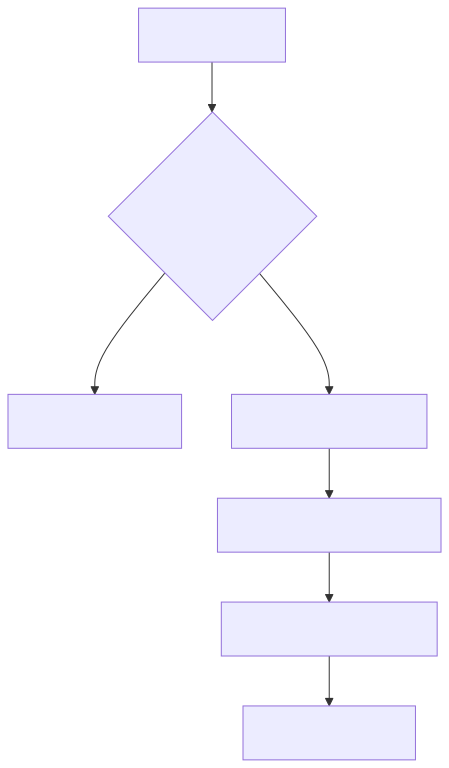
\includegraphics[keepaspectratio,alt={Diagram 7}]{diagrams/tour-07.pdf}}
\caption{Diagram 7}
\end{figure}

\textbf{The Footprint}: A declaration of what resources the rule will
read and write:

\begin{Shaded}
\begin{Highlighting}[]
\KeywordTok{pub} \KeywordTok{struct}\NormalTok{ Footprint }\OperatorTok{\{}
    \KeywordTok{pub}\NormalTok{ n\_read}\OperatorTok{:}\NormalTok{ BTreeSet}\OperatorTok{\textless{}}\NormalTok{NodeId}\OperatorTok{\textgreater{},}   \CommentTok{// Nodes to read}
    \KeywordTok{pub}\NormalTok{ n\_write}\OperatorTok{:}\NormalTok{ BTreeSet}\OperatorTok{\textless{}}\NormalTok{NodeId}\OperatorTok{\textgreater{},}  \CommentTok{// Nodes to write}
    \KeywordTok{pub}\NormalTok{ e\_read}\OperatorTok{:}\NormalTok{ BTreeSet}\OperatorTok{\textless{}}\NormalTok{EdgeId}\OperatorTok{\textgreater{},}   \CommentTok{// Edges to read}
    \KeywordTok{pub}\NormalTok{ e\_write}\OperatorTok{:}\NormalTok{ BTreeSet}\OperatorTok{\textless{}}\NormalTok{EdgeId}\OperatorTok{\textgreater{},}  \CommentTok{// Edges to write}
    \KeywordTok{pub}\NormalTok{ a\_read}\OperatorTok{:}\NormalTok{ BTreeSet}\OperatorTok{\textless{}}\NormalTok{AttachmentKey}\OperatorTok{\textgreater{},}  \CommentTok{// Attachments to read}
    \KeywordTok{pub}\NormalTok{ a\_write}\OperatorTok{:}\NormalTok{ BTreeSet}\OperatorTok{\textless{}}\NormalTok{AttachmentKey}\OperatorTok{\textgreater{},} \CommentTok{// Attachments to write}
    \CommentTok{// ... ports, factor\_mask}
\OperatorTok{\}}
\end{Highlighting}
\end{Shaded}

\textbf{Scheduler deduplication}: If the same
\texttt{(scope\_hash,\ rule\_id)} is applied multiple times,
\textbf{last wins}. This enables idempotent retry semantics.

\subsection{5.4 Phase 3: Commit (The Heart of
Determinism)}\label{phase-3-commit-the-heart-of-determinism}

\begin{Shaded}
\begin{Highlighting}[]
\KeywordTok{let}\NormalTok{ (snapshot}\OperatorTok{,}\NormalTok{ receipt}\OperatorTok{,}\NormalTok{ patch) }\OperatorTok{=}\NormalTok{ engine}\OperatorTok{.}\NormalTok{commit\_with\_receipt(tx)}\OperatorTok{;}
\end{Highlighting}
\end{Shaded}

This is where Echo's magic happens. Let's break it down:

\subsubsection{5.4.1 Drain}\label{drain}

The scheduler drains all pending rewrites in \textbf{canonical order}:

\begin{Shaded}
\begin{Highlighting}[]
\CommentTok{// RadixScheduler uses O(n) LSD radix sort}
\CommentTok{// 20 passes: 2 nonce + 2 rule\_id + 16 scope\_hash (16{-}bit digits)}
\KeywordTok{let}\NormalTok{ rewrites }\OperatorTok{=}\NormalTok{ scheduler}\OperatorTok{.}\NormalTok{drain\_for\_tx(tx)}\OperatorTok{;}  \CommentTok{// Vec\textless{}PendingRewrite\textgreater{} in canonical order}
\end{Highlighting}
\end{Shaded}

\textbf{Ordering key}:
\texttt{(scope\_hash{[}0..32{]},\ rule\_id,\ nonce)}

This ensures the \textbf{same rewrites always execute in the same
order}, regardless of when they were applied.

\begin{claudecommentary}
**Claude's Take**: Radix sort! They're using radix sort for the scheduler drain. Not quicksort, not merge sort—radix sort.

Why? Because radix sort is *stable* and *deterministic* by construction. Quicksort's behavior depends on pivot selection, which can vary. Merge sort is deterministic, but radix sort is faster for fixed-size keys. Since the ordering key is exactly 36 bytes (32-byte scope hash + 2-byte rule ID + 2-byte nonce), radix sort is perfect.

This is the kind of detail that separates "deterministic by accident" from "deterministic by design."
\end{claudecommentary}

\subsubsection{5.4.2 Reserve (Independence
Check)}\label{reserve-independence-check}

For each rewrite in canonical order:

\begin{figure}
\centering
\pandocbounded{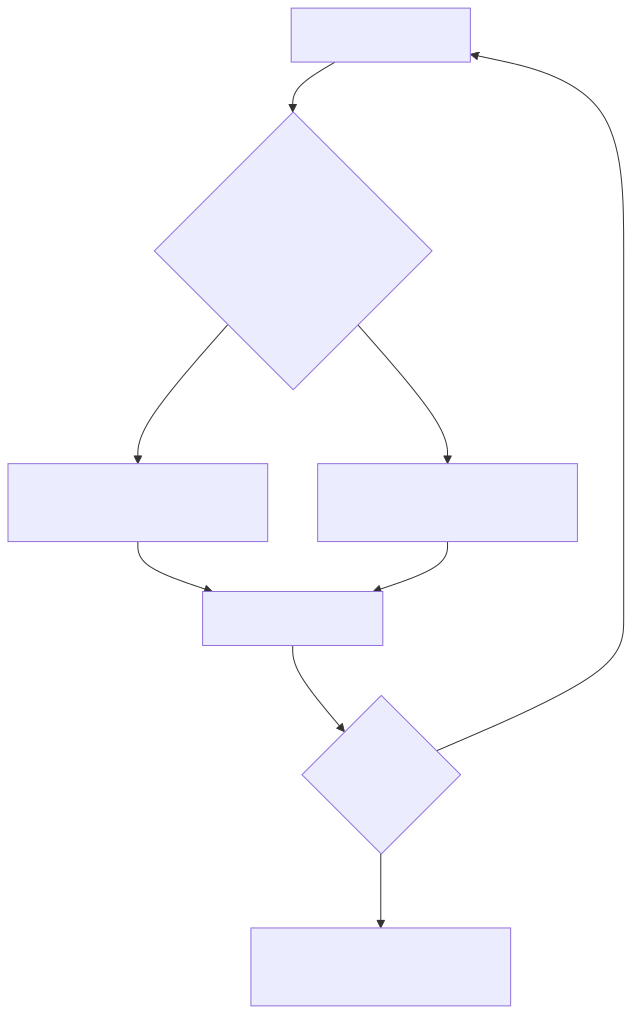
\includegraphics[keepaspectratio,alt={Diagram 8}]{diagrams/tour-08.pdf}}
\caption{Diagram 8}
\end{figure}

\textbf{Conflict detection}: Uses
\texttt{GenSet\textless{}K\textgreater{}} for O(1) lookups: - Read-read
overlap: \textbf{allowed} - Write-write overlap: \textbf{conflict} -
Read-write overlap: \textbf{conflict}

\subsubsection{5.4.3 Execute (Parallel,
Lockless)}\label{execute-parallel-lockless}

Accepted rewrites execute against the \textbf{read-only snapshot}:

\begin{Shaded}
\begin{Highlighting}[]
\ControlFlowTok{for}\NormalTok{ rewrite }\KeywordTok{in}\NormalTok{ accepted }\OperatorTok{\{}
    \KeywordTok{let}\NormalTok{ rule }\OperatorTok{=} \OperatorTok{\&}\NormalTok{rules[rewrite}\OperatorTok{.}\NormalTok{rule\_id]}\OperatorTok{;}
    \KeywordTok{let}\NormalTok{ view }\OperatorTok{=} \PreprocessorTok{GraphView::}\NormalTok{new(}\OperatorTok{\&}\NormalTok{state}\OperatorTok{,}\NormalTok{ rewrite}\OperatorTok{.}\NormalTok{warp\_id)}\OperatorTok{;}

    \CommentTok{// Executor reads from view, emits to delta}
\NormalTok{    (rule}\OperatorTok{.}\NormalTok{executor)(view}\OperatorTok{,} \OperatorTok{\&}\NormalTok{rewrite}\OperatorTok{.}\NormalTok{scope}\OperatorTok{,} \OperatorTok{\&}\KeywordTok{mut}\NormalTok{ delta)}\OperatorTok{;}
\OperatorTok{\}}
\end{Highlighting}
\end{Shaded}

\textbf{Critical}: \texttt{GraphView} is immutable. \texttt{TickDelta}
accumulates operations:

\begin{Shaded}
\begin{Highlighting}[]
\KeywordTok{pub} \KeywordTok{struct}\NormalTok{ TickDelta }\OperatorTok{\{}
\NormalTok{    ops}\OperatorTok{:} \DataTypeTok{Vec}\OperatorTok{\textless{}}\NormalTok{(WarpOp}\OperatorTok{,}\NormalTok{ OpOrigin)}\OperatorTok{\textgreater{},}
\OperatorTok{\}}

\CommentTok{// Operations emitted during execution:}
\NormalTok{delta}\OperatorTok{.}\NormalTok{emit(}\PreprocessorTok{WarpOp::}\NormalTok{UpsertNode }\OperatorTok{\{}\NormalTok{ id}\OperatorTok{,}\NormalTok{ record }\OperatorTok{\}}\NormalTok{)}\OperatorTok{;}
\NormalTok{delta}\OperatorTok{.}\NormalTok{emit(}\PreprocessorTok{WarpOp::}\NormalTok{UpsertEdge }\OperatorTok{\{}\NormalTok{ from}\OperatorTok{,}\NormalTok{ edge }\OperatorTok{\}}\NormalTok{)}\OperatorTok{;}
\NormalTok{delta}\OperatorTok{.}\NormalTok{emit(}\PreprocessorTok{WarpOp::}\NormalTok{DeleteNode }\OperatorTok{\{}\NormalTok{ id }\OperatorTok{\}}\NormalTok{)}\OperatorTok{;}
\NormalTok{delta}\OperatorTok{.}\NormalTok{emit(}\PreprocessorTok{WarpOp::}\NormalTok{SetAttachment }\OperatorTok{\{}\NormalTok{ node}\OperatorTok{,}\NormalTok{ key}\OperatorTok{,}\NormalTok{ value }\OperatorTok{\}}\NormalTok{)}\OperatorTok{;}
\end{Highlighting}
\end{Shaded}

\subsubsection{5.4.4 Merge (Canonical Sort)}\label{merge-canonical-sort}

All operations are sorted into \textbf{canonical replay order}:

\begin{Shaded}
\begin{Highlighting}[]
\CommentTok{// Sort by (WarpOpKey, OpOrigin)}
\NormalTok{ops}\OperatorTok{.}\NormalTok{sort\_by\_key(}\OperatorTok{|}\NormalTok{(op}\OperatorTok{,}\NormalTok{ origin)}\OperatorTok{|}\NormalTok{ (op}\OperatorTok{.}\NormalTok{sort\_key()}\OperatorTok{,}\NormalTok{ origin}\OperatorTok{.}\NormalTok{clone()))}\OperatorTok{;}

\CommentTok{// Deduplicate identical ops}
\CommentTok{// Error on conflicting ops (footprint model violation)}
\end{Highlighting}
\end{Shaded}

\textbf{Conflict handling}: If two rewrites wrote \textbf{different
values} to the same key, that's a bug in the footprint model. Echo
errors loudly.

\subsubsection{5.4.5 Finalize}\label{finalize}

Apply the merged delta to produce the new state:

\begin{Shaded}
\begin{Highlighting}[]
\ControlFlowTok{for}\NormalTok{ op }\KeywordTok{in}\NormalTok{ merged\_ops }\OperatorTok{\{}
    \ControlFlowTok{match}\NormalTok{ op }\OperatorTok{\{}
        \PreprocessorTok{WarpOp::}\NormalTok{UpsertNode }\OperatorTok{\{}\NormalTok{ id}\OperatorTok{,}\NormalTok{ record }\OperatorTok{\}} \OperatorTok{=\textgreater{}}\NormalTok{ state}\OperatorTok{.}\NormalTok{insert\_node(id}\OperatorTok{,}\NormalTok{ record)}\OperatorTok{,}
        \PreprocessorTok{WarpOp::}\NormalTok{UpsertEdge }\OperatorTok{\{}\NormalTok{ from}\OperatorTok{,}\NormalTok{ edge }\OperatorTok{\}} \OperatorTok{=\textgreater{}}\NormalTok{ state}\OperatorTok{.}\NormalTok{insert\_edge(from}\OperatorTok{,}\NormalTok{ edge)}\OperatorTok{,}
        \PreprocessorTok{WarpOp::}\NormalTok{DeleteNode }\OperatorTok{\{}\NormalTok{ id }\OperatorTok{\}} \OperatorTok{=\textgreater{}}\NormalTok{ state}\OperatorTok{.}\NormalTok{delete\_node\_cascade(id)}\OperatorTok{,}
        \PreprocessorTok{WarpOp::}\NormalTok{SetAttachment }\OperatorTok{\{}\NormalTok{ node}\OperatorTok{,}\NormalTok{ key}\OperatorTok{,}\NormalTok{ value }\OperatorTok{\}} \OperatorTok{=\textgreater{}}\NormalTok{ state}\OperatorTok{.}\NormalTok{set\_attachment(node}\OperatorTok{,}\NormalTok{ key}\OperatorTok{,}\NormalTok{ value)}\OperatorTok{,}
        \CommentTok{// ...}
    \OperatorTok{\}}
\OperatorTok{\}}
\end{Highlighting}
\end{Shaded}

\subsection{5.5 Phase 4: Hash
Computation}\label{phase-4-hash-computation}

\subsubsection{State Root (BLAKE3)}\label{state-root-blake3}

The state root is computed via \textbf{deterministic BFS} over reachable
nodes:

\begin{figure}
\centering
\pandocbounded{\includegraphics[keepaspectratio,alt={Diagram 9}]{diagrams/tour-09.pdf}}
\caption{Diagram 9}
\end{figure}

\textbf{Encoding} (architecture-independent): - All IDs: raw 32 bytes -
Counts: u64 little-endian - Payloads: 1-byte tag + type\_id{[}32{]} +
u64 LE length + bytes

\subsubsection{Commit Hash (v2)}\label{commit-hash-v2}

\begin{Shaded}
\begin{Highlighting}[]
\NormalTok{commit\_hash }\OperatorTok{=}\NormalTok{ BLAKE3(}
\NormalTok{    version\_tag[}\DecValTok{4}\NormalTok{]      }\OperatorTok{||}  \CommentTok{// Protocol version}
\NormalTok{    parents[]           }\OperatorTok{||}  \CommentTok{// Parent commit hashes}
\NormalTok{    state\_root[}\DecValTok{32}\NormalTok{]      }\OperatorTok{||}  \CommentTok{// Graph{-}only hash}
\NormalTok{    patch\_digest[}\DecValTok{32}\NormalTok{]    }\OperatorTok{||}  \CommentTok{// Merged ops digest}
\NormalTok{    policy\_id[}\DecValTok{4}\NormalTok{]            }\CommentTok{// Policy identifier}
\NormalTok{)}
\end{Highlighting}
\end{Shaded}

\begin{claudecommentary}
**Claude's Take**: The commit hash includes a `policy_id`. This is subtle but important: two engines with different policies could produce the same state but different commit hashes. Why? Because the *process* matters, not just the result.

Imagine one policy allows rules to run in parallel; another requires sequential execution. They might produce identical graphs, but the commit hashes differ because the policies differ. This prevents accidentally mixing outputs from incompatible engine configurations.

It's defensive design: "Trust, but verify—and make verification easy."
\end{claudecommentary}

\subsection{5.6 Phase 5: Record to
History}\label{phase-5-record-to-history}

\begin{Shaded}
\begin{Highlighting}[]
\NormalTok{history}\OperatorTok{.}\NormalTok{push((}
\NormalTok{    Snapshot }\OperatorTok{\{}\NormalTok{ hash}\OperatorTok{:}\NormalTok{ commit\_hash}\OperatorTok{,}\NormalTok{ state\_root}\OperatorTok{,}\NormalTok{ parents}\OperatorTok{,} \OperatorTok{...} \OperatorTok{\},}
\NormalTok{    TickReceipt }\OperatorTok{\{}\NormalTok{ applied}\OperatorTok{,}\NormalTok{ rejected}\OperatorTok{,} \OperatorTok{...} \OperatorTok{\},}
\NormalTok{    WarpTickPatchV1 }\OperatorTok{\{}\NormalTok{ ops}\OperatorTok{,}\NormalTok{ in\_slots}\OperatorTok{,}\NormalTok{ out\_slots}\OperatorTok{,}\NormalTok{ patch\_digest}\OperatorTok{,} \OperatorTok{...} \OperatorTok{\}}
\NormalTok{))}\OperatorTok{;}
\end{Highlighting}
\end{Shaded}

The patch is \textbf{prescriptive}: it can be replayed without
re-matching to reproduce the exact same state.

\begin{center}\rule{0.5\linewidth}{0.5pt}\end{center}

\section{6. Parallel Execution: BOAW (Bag of Autonomous
Workers)}\label{parallel-execution-boaw-bag-of-autonomous-workers}

\subsection{6.1 What is BOAW?}\label{what-is-boaw}

BOAW stands for \textbf{Bag of Autonomous Workers}. It's Echo's parallel
execution architecture that enables:

\begin{itemize}
\tightlist
\item
  \textbf{Massive parallelism} without locks
\item
  \textbf{Deterministic convergence} across platforms
\item
  \textbf{Worker-count invariance} (same result with 1 or 32 workers)
\end{itemize}

\subsection{6.2 The Key Insight}\label{the-key-insight}

\begin{verbatim}
┌──────────────────────────────────────────────────────────────────┐
│                    THE BOAW INSIGHT                               │
├──────────────────────────────────────────────────────────────────┤
│                                                                   │
│  Traditional parallelism:                                         │
│    "Make execution order deterministic" → Complex, slow           │
│                                                                   │
│  BOAW parallelism:                                                │
│    "Let execution order vary, make MERGE deterministic" → Fast!   │
│                                                                   │
│  Workers race freely → Each produces a TickDelta                  │
│  Merge step sorts all deltas → Canonical output                   │
│                                                                   │
└──────────────────────────────────────────────────────────────────┘
\end{verbatim}

\begin{claudecommentary}
**Claude's Take**: This is the insight that makes Echo work. Most parallel systems try to *control* the execution order—barriers, locks, atomic sequences. BOAW says: "Forget it. Let chaos reign during execution. We'll sort it out in the merge."

It's like MapReduce: the map phase runs in any order; the reduce phase (merge) produces the canonical result. But unlike MapReduce, Echo operates on a graph with complex dependencies. The footprint model makes this possible: by declaring what you'll touch before executing, you enable the merge to validate that no conflicts occurred.

If this sounds too good to be true, it mostly is—*if* you get the footprints wrong. The system is only as deterministic as your footprint declarations. Lie to the footprint system, and you'll get non-determinism.
\end{claudecommentary}

\subsection{6.3 Execution Strategies}\label{execution-strategies}

\subsubsection{Phase 6A: Stride Partitioning
(Legacy)}\label{phase-6a-stride-partitioning-legacy}

\begin{verbatim}
Worker 0: items[0], items[4], items[8], ...
Worker 1: items[1], items[5], items[9], ...
Worker 2: items[2], items[6], items[10], ...
Worker 3: items[3], items[7], items[11], ...
\end{verbatim}

\textbf{Problem}: Poor cache locality---related items scatter across
workers.

\subsubsection{Phase 6B: Virtual Shards (Current
Default)}\label{phase-6b-virtual-shards-current-default}

\begin{Shaded}
\begin{Highlighting}[]
\KeywordTok{const}\NormalTok{ NUM\_SHARDS}\OperatorTok{:} \DataTypeTok{usize} \OperatorTok{=} \DecValTok{256}\OperatorTok{;}  \CommentTok{// Protocol constant (frozen)}

\KeywordTok{fn}\NormalTok{ shard\_of(node\_id}\OperatorTok{:} \OperatorTok{\&}\NormalTok{NodeId) }\OperatorTok{{-}\textgreater{}} \DataTypeTok{usize} \OperatorTok{\{}
    \KeywordTok{let}\NormalTok{ bytes }\OperatorTok{=}\NormalTok{ node\_id}\OperatorTok{.}\NormalTok{as\_bytes()}\OperatorTok{;}
    \KeywordTok{let}\NormalTok{ val }\OperatorTok{=} \DataTypeTok{u64}\PreprocessorTok{::}\NormalTok{from\_le\_bytes(bytes[}\DecValTok{0}\OperatorTok{..}\DecValTok{8}\NormalTok{])}\OperatorTok{;}
\NormalTok{    (val }\OperatorTok{\&} \DecValTok{255}\NormalTok{) }\KeywordTok{as} \DataTypeTok{usize}  \CommentTok{// Fast modulo via bitmask}
\OperatorTok{\}}
\end{Highlighting}
\end{Shaded}

\begin{figure}
\centering
\pandocbounded{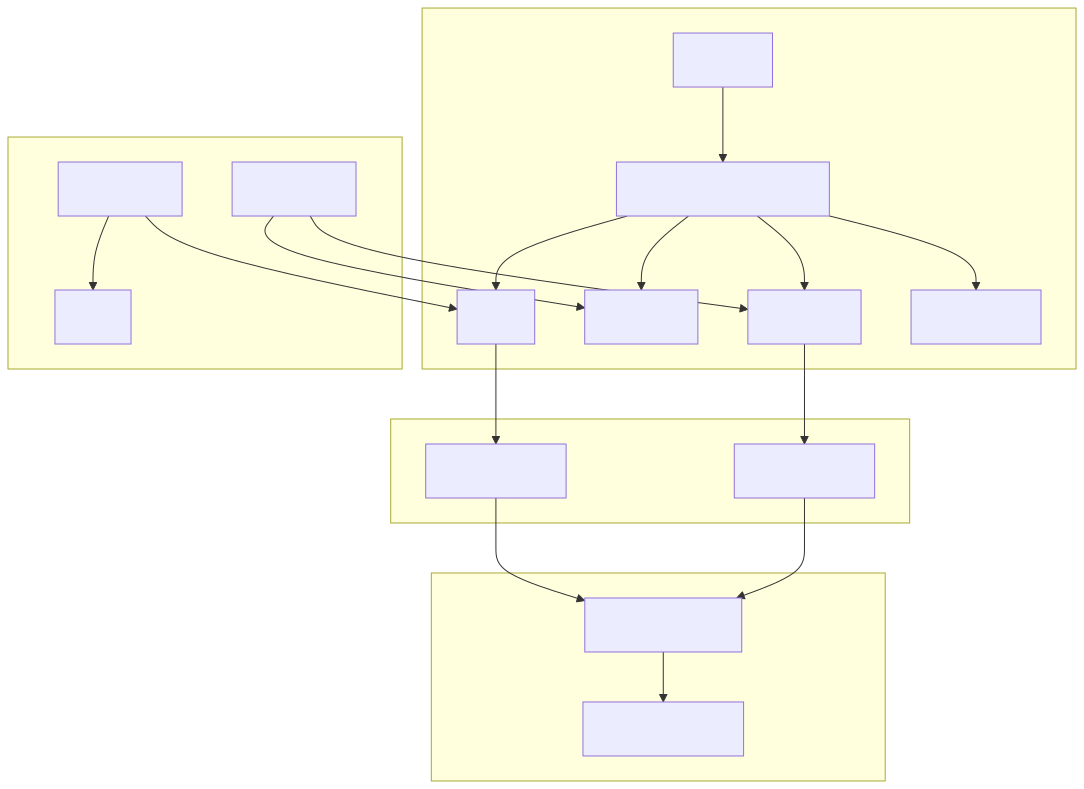
\includegraphics[keepaspectratio,alt={Diagram 10}]{diagrams/tour-10.pdf}}
\caption{Diagram 10}
\end{figure}

\textbf{Benefits}: - Items with same \texttt{shard\_of(scope)} processed
together → better cache hits - Workers dynamically claim shards via
atomic counter → load balancing - Determinism enforced by merge, not
execution order

\begin{claudecommentary}
**Claude's Take**: 256 shards is an interesting choice. It's small enough that the atomic counter for work-stealing doesn't become a bottleneck, but large enough to distribute work across many cores.

The `& 255` bitmask is a micro-optimization I appreciate. It's equivalent to `% 256` but faster because 256 is a power of 2. This is the kind of low-level detail that adds up when you're processing millions of items per second.

One thing I wondered: what if your NodeIds are clustered? Like, if all recent nodes have IDs starting with `0x00...`, they'd all end up in shard 0. I suspect content-addressed IDs (via BLAKE3) distribute uniformly, so this isn't a problem in practice. But for user-assigned IDs, you'd need to be careful.
\end{claudecommentary}

\subsection{6.4 The Execution Loop}\label{the-execution-loop}

\begin{Shaded}
\begin{Highlighting}[]
\KeywordTok{pub} \KeywordTok{fn}\NormalTok{ execute\_parallel\_sharded(}
\NormalTok{    view}\OperatorTok{:}\NormalTok{ GraphView}\OperatorTok{\textless{}}\OtherTok{\textquotesingle{}\_}\OperatorTok{\textgreater{},}
\NormalTok{    items}\OperatorTok{:} \OperatorTok{\&}\NormalTok{[ExecItem]}\OperatorTok{,}
\NormalTok{    workers}\OperatorTok{:} \DataTypeTok{usize}\OperatorTok{,}
\NormalTok{) }\OperatorTok{{-}\textgreater{}} \DataTypeTok{Vec}\OperatorTok{\textless{}}\NormalTok{TickDelta}\OperatorTok{\textgreater{}} \OperatorTok{\{}
    \CommentTok{// Partition items into 256 shards}
    \KeywordTok{let}\NormalTok{ shards }\OperatorTok{=}\NormalTok{ partition\_into\_shards(items)}\OperatorTok{;}

    \CommentTok{// Atomic counter for work{-}stealing}
    \KeywordTok{let}\NormalTok{ next\_shard }\OperatorTok{=} \PreprocessorTok{AtomicUsize::}\NormalTok{new(}\DecValTok{0}\NormalTok{)}\OperatorTok{;}

    \PreprocessorTok{std::thread::}\NormalTok{scope(}\OperatorTok{|}\NormalTok{s}\OperatorTok{|} \OperatorTok{\{}
        \KeywordTok{let}\NormalTok{ handles}\OperatorTok{:} \DataTypeTok{Vec}\OperatorTok{\textless{}}\NormalTok{\_}\OperatorTok{\textgreater{}} \OperatorTok{=}\NormalTok{ (}\DecValTok{0}\OperatorTok{..}\NormalTok{workers)}\OperatorTok{.}\NormalTok{map(}\OperatorTok{|}\NormalTok{\_}\OperatorTok{|} \OperatorTok{\{}
\NormalTok{            s}\OperatorTok{.}\NormalTok{spawn(}\OperatorTok{||} \OperatorTok{\{}
                \KeywordTok{let} \KeywordTok{mut}\NormalTok{ delta }\OperatorTok{=} \PreprocessorTok{TickDelta::}\NormalTok{new()}\OperatorTok{;}
                \ControlFlowTok{loop} \OperatorTok{\{}
                    \CommentTok{// Claim next shard atomically}
                    \KeywordTok{let}\NormalTok{ shard\_id }\OperatorTok{=}\NormalTok{ next\_shard}\OperatorTok{.}\NormalTok{fetch\_add(}\DecValTok{1}\OperatorTok{,} \PreprocessorTok{Ordering::}\NormalTok{Relaxed)}\OperatorTok{;}
                    \ControlFlowTok{if}\NormalTok{ shard\_id }\OperatorTok{\textgreater{}=}\NormalTok{ NUM\_SHARDS }\OperatorTok{\{} \ControlFlowTok{break}\OperatorTok{;} \OperatorTok{\}}

                    \CommentTok{// Execute all items in this shard}
                    \ControlFlowTok{for}\NormalTok{ item }\KeywordTok{in} \OperatorTok{\&}\NormalTok{shards[shard\_id]}\OperatorTok{.}\NormalTok{items }\OperatorTok{\{}
\NormalTok{                        (item}\OperatorTok{.}\NormalTok{exec)(view}\OperatorTok{.}\NormalTok{clone()}\OperatorTok{,} \OperatorTok{\&}\NormalTok{item}\OperatorTok{.}\NormalTok{scope}\OperatorTok{,} \OperatorTok{\&}\KeywordTok{mut}\NormalTok{ delta)}\OperatorTok{;}
                    \OperatorTok{\}}
                \OperatorTok{\}}
\NormalTok{                delta}
            \OperatorTok{\}}\NormalTok{)}
        \OperatorTok{\}}\NormalTok{)}\OperatorTok{.}\NormalTok{collect()}\OperatorTok{;}

\NormalTok{        handles}\OperatorTok{.}\NormalTok{into\_iter()}\OperatorTok{.}\NormalTok{map(}\OperatorTok{|}\NormalTok{h}\OperatorTok{|}\NormalTok{ h}\OperatorTok{.}\NormalTok{join()}\OperatorTok{.}\NormalTok{unwrap())}\OperatorTok{.}\NormalTok{collect()}
    \OperatorTok{\}}\NormalTok{)}
\OperatorTok{\}}
\end{Highlighting}
\end{Shaded}

\subsection{6.5 The Canonical Merge}\label{the-canonical-merge}

\begin{Shaded}
\begin{Highlighting}[]
\KeywordTok{pub} \KeywordTok{fn}\NormalTok{ merge\_deltas(deltas}\OperatorTok{:} \DataTypeTok{Vec}\OperatorTok{\textless{}}\NormalTok{TickDelta}\OperatorTok{\textgreater{}}\NormalTok{) }\OperatorTok{{-}\textgreater{}} \DataTypeTok{Result}\OperatorTok{\textless{}}\DataTypeTok{Vec}\OperatorTok{\textless{}}\NormalTok{WarpOp}\OperatorTok{\textgreater{},}\NormalTok{ MergeConflict}\OperatorTok{\textgreater{}} \OperatorTok{\{}
    \CommentTok{// 1. Flatten all ops from all workers}
    \KeywordTok{let} \KeywordTok{mut}\NormalTok{ all\_ops}\OperatorTok{:} \DataTypeTok{Vec}\OperatorTok{\textless{}}\NormalTok{(WarpOpKey}\OperatorTok{,}\NormalTok{ OpOrigin}\OperatorTok{,}\NormalTok{ WarpOp)}\OperatorTok{\textgreater{}} \OperatorTok{=}\NormalTok{ deltas}
        \OperatorTok{.}\NormalTok{into\_iter()}
        \OperatorTok{.}\NormalTok{flat\_map(}\OperatorTok{|}\NormalTok{d}\OperatorTok{|}\NormalTok{ d}\OperatorTok{.}\NormalTok{ops\_with\_origins())}
        \OperatorTok{.}\NormalTok{collect()}\OperatorTok{;}

    \CommentTok{// 2. Sort canonically by (key, origin)}
\NormalTok{    all\_ops}\OperatorTok{.}\NormalTok{sort\_by\_key(}\OperatorTok{|}\NormalTok{(key}\OperatorTok{,}\NormalTok{ origin}\OperatorTok{,}\NormalTok{ \_)}\OperatorTok{|}\NormalTok{ (key}\OperatorTok{.}\NormalTok{clone()}\OperatorTok{,}\NormalTok{ origin}\OperatorTok{.}\NormalTok{clone()))}\OperatorTok{;}

    \CommentTok{// 3. Deduplicate and detect conflicts}
    \KeywordTok{let} \KeywordTok{mut}\NormalTok{ result }\OperatorTok{=} \DataTypeTok{Vec}\PreprocessorTok{::}\NormalTok{new()}\OperatorTok{;}
    \ControlFlowTok{for}\NormalTok{ group }\KeywordTok{in}\NormalTok{ all\_ops}\OperatorTok{.}\NormalTok{group\_by(}\OperatorTok{|}\NormalTok{(k1}\OperatorTok{,}\NormalTok{ \_}\OperatorTok{,}\NormalTok{ \_)}\OperatorTok{,}\NormalTok{ (k2}\OperatorTok{,}\NormalTok{ \_}\OperatorTok{,}\NormalTok{ \_)}\OperatorTok{|}\NormalTok{ k1 }\OperatorTok{==}\NormalTok{ k2) }\OperatorTok{\{}
        \KeywordTok{let}\NormalTok{ first }\OperatorTok{=} \OperatorTok{\&}\NormalTok{group[}\DecValTok{0}\NormalTok{]}\OperatorTok{.}\DecValTok{2}\OperatorTok{;}
        \ControlFlowTok{if}\NormalTok{ group}\OperatorTok{.}\NormalTok{iter()}\OperatorTok{.}\NormalTok{all(}\OperatorTok{|}\NormalTok{(\_}\OperatorTok{,}\NormalTok{ \_}\OperatorTok{,}\NormalTok{ op)}\OperatorTok{|}\NormalTok{ op }\OperatorTok{==}\NormalTok{ first) }\OperatorTok{\{}
\NormalTok{            result}\OperatorTok{.}\NormalTok{push(first}\OperatorTok{.}\NormalTok{clone())}\OperatorTok{;}  \CommentTok{// All identical: keep one}
        \OperatorTok{\}} \ControlFlowTok{else} \OperatorTok{\{}
            \ControlFlowTok{return} \ConstantTok{Err}\NormalTok{(MergeConflict }\OperatorTok{\{}\NormalTok{ writers}\OperatorTok{:}\NormalTok{ group}\OperatorTok{.}\NormalTok{iter()}\OperatorTok{.}\NormalTok{map(}\OperatorTok{|}\NormalTok{(\_}\OperatorTok{,}\NormalTok{ o}\OperatorTok{,}\NormalTok{ \_)}\OperatorTok{|}\NormalTok{ o)}\OperatorTok{.}\NormalTok{collect() }\OperatorTok{\}}\NormalTok{)}\OperatorTok{;}
        \OperatorTok{\}}
    \OperatorTok{\}}

    \ConstantTok{Ok}\NormalTok{(result)}
\OperatorTok{\}}
\end{Highlighting}
\end{Shaded}

\textbf{Key guarantee}: Conflicts are bugs. If footprints were correct,
no two rewrites should write different values to the same key.

\begin{center}\rule{0.5\linewidth}{0.5pt}\end{center}

\section{7. Storage \& Hashing: Content-Addressed
Truth}\label{storage-hashing-content-addressed-truth}

\subsection{7.1 The GraphStore}\label{the-graphstore}

Located in \texttt{crates/warp-core/src/graph.rs}:

\begin{Shaded}
\begin{Highlighting}[]
\KeywordTok{pub} \KeywordTok{struct}\NormalTok{ GraphStore }\OperatorTok{\{}
    \KeywordTok{pub}\NormalTok{(}\KeywordTok{crate}\NormalTok{) warp\_id}\OperatorTok{:}\NormalTok{ WarpId}\OperatorTok{,}
    \KeywordTok{pub}\NormalTok{(}\KeywordTok{crate}\NormalTok{) nodes}\OperatorTok{:}\NormalTok{ BTreeMap}\OperatorTok{\textless{}}\NormalTok{NodeId}\OperatorTok{,}\NormalTok{ NodeRecord}\OperatorTok{\textgreater{},}
    \KeywordTok{pub}\NormalTok{(}\KeywordTok{crate}\NormalTok{) edges\_from}\OperatorTok{:}\NormalTok{ BTreeMap}\OperatorTok{\textless{}}\NormalTok{NodeId}\OperatorTok{,} \DataTypeTok{Vec}\OperatorTok{\textless{}}\NormalTok{EdgeRecord}\OperatorTok{\textgreater{}\textgreater{},}
    \KeywordTok{pub}\NormalTok{(}\KeywordTok{crate}\NormalTok{) edges\_to}\OperatorTok{:}\NormalTok{ BTreeMap}\OperatorTok{\textless{}}\NormalTok{NodeId}\OperatorTok{,} \DataTypeTok{Vec}\OperatorTok{\textless{}}\NormalTok{EdgeId}\OperatorTok{\textgreater{}\textgreater{},}  \CommentTok{// Reverse index}
    \KeywordTok{pub}\NormalTok{(}\KeywordTok{crate}\NormalTok{) node\_attachments}\OperatorTok{:}\NormalTok{ BTreeMap}\OperatorTok{\textless{}}\NormalTok{NodeId}\OperatorTok{,}\NormalTok{ AttachmentValue}\OperatorTok{\textgreater{},}
    \KeywordTok{pub}\NormalTok{(}\KeywordTok{crate}\NormalTok{) edge\_attachments}\OperatorTok{:}\NormalTok{ BTreeMap}\OperatorTok{\textless{}}\NormalTok{EdgeId}\OperatorTok{,}\NormalTok{ AttachmentValue}\OperatorTok{\textgreater{},}
    \KeywordTok{pub}\NormalTok{(}\KeywordTok{crate}\NormalTok{) edge\_index}\OperatorTok{:}\NormalTok{ BTreeMap}\OperatorTok{\textless{}}\NormalTok{EdgeId}\OperatorTok{,}\NormalTok{ NodeId}\OperatorTok{\textgreater{},}     \CommentTok{// Edge → Source}
    \KeywordTok{pub}\NormalTok{(}\KeywordTok{crate}\NormalTok{) edge\_to\_index}\OperatorTok{:}\NormalTok{ BTreeMap}\OperatorTok{\textless{}}\NormalTok{EdgeId}\OperatorTok{,}\NormalTok{ NodeId}\OperatorTok{\textgreater{},}  \CommentTok{// Edge → Target}
\OperatorTok{\}}
\end{Highlighting}
\end{Shaded}

\textbf{Why BTreeMap everywhere?} - Deterministic iteration order
(sorted by key) - Enables canonical hashing - No HashMap ordering
surprises

\begin{claudecommentary}
**Claude's Take**: Seven BTreeMaps! This is the price of determinism. Each of these maps is sorted, which means:

1. Insertions are O(log n) instead of O(1) amortized for HashMap
2. Iteration is always in key order, so hashing is deterministic
3. Memory overhead is slightly higher due to tree structure

Is it worth it? For Echo's use case, absolutely. The alternative—using HashMap and then sorting before each hash—would be slower and more error-prone. By paying the cost upfront (O(log n) writes), you get guaranteed correctness.

The multiple indices (`edges_from`, `edges_to`, `edge_index`, `edge_to_index`) look redundant, but they enable O(log n) lookups from any direction. Want all edges *from* a node? `edges_from[node_id]`. Want all edges *to* a node? `edges_to[node_id]`. This is a classic space-time tradeoff.
\end{claudecommentary}

\subsection{7.2 WSC: Write-Streaming Columnar
Format}\label{wsc-write-streaming-columnar-format}

For efficient snapshots, Echo uses WSC---a zero-copy, mmap-friendly
format:

\begin{verbatim}
┌─────────────────────────────────────────────────────────────────┐
│ WSC SNAPSHOT FILE                                                │
├─────────────────────────────────────────────────────────────────┤
│ ┌─────────────────────────────────────────────────────────────┐ │
│ │ NODES TABLE (sorted by NodeId)                              │ │
│ │ ┌──────────┬───────────┬──────────┐                        │ │
│ │ │ NodeRow  │ NodeRow   │ NodeRow  │ ...                    │ │
│ │ │ 64 bytes │ 64 bytes  │ 64 bytes │                        │ │
│ │ └──────────┴───────────┴──────────┘                        │ │
│ └─────────────────────────────────────────────────────────────┘ │
│ ┌─────────────────────────────────────────────────────────────┐ │
│ │ EDGES TABLE (sorted by EdgeId)                              │ │
│ │ ┌───────────┬───────────┬───────────┐                      │ │
│ │ │ EdgeRow   │ EdgeRow   │ EdgeRow   │ ...                  │ │
│ │ │ 128 bytes │ 128 bytes │ 128 bytes │                      │ │
│ │ └───────────┴───────────┴───────────┘                      │ │
│ └─────────────────────────────────────────────────────────────┘ │
│ ┌─────────────────────────────────────────────────────────────┐ │
│ │ OUT_INDEX (per-node → range into out_edges)                 │ │
│ │ ┌────────────────┬────────────────┐                        │ │
│ │ │ Range (16 B)   │ Range (16 B)   │ ...                    │ │
│ │ └────────────────┴────────────────┘                        │ │
│ └─────────────────────────────────────────────────────────────┘ │
│ ┌─────────────────────────────────────────────────────────────┐ │
│ │ BLOB ARENA (variable-length data)                           │ │
│ │ Referenced by (offset, length) tuples                       │ │
│ └─────────────────────────────────────────────────────────────┘ │
└─────────────────────────────────────────────────────────────────┘
\end{verbatim}

\textbf{Row types} (8-byte aligned): - \texttt{NodeRow}: 64 bytes
(node\_id{[}32{]} + node\_type{[}32{]}) - \texttt{EdgeRow}: 128 bytes
(edge\_id{[}32{]} + from{[}32{]} + to{[}32{]} + type{[}32{]}) -
\texttt{Range}: 16 bytes (start\_le{[}8{]} + len\_le{[}8{]})

\begin{claudecommentary}
**Claude's Take**: WSC is gloriously simple. Fixed-size rows, sorted tables, binary search for lookups. No compression, no Parquet-style encoding tricks—just flat bytes on disk that you can mmap and use directly.

The trade-off is size: WSC files are larger than compressed formats. But the benefit is speed: you can find node #1000 by seeking to `offset + 1000 * 64` and reading 64 bytes. No decompression, no index lookups, no memory allocation.

For Echo's use case (local caching, fast restarts), this makes sense. You're not storing petabytes; you're storing the state of a single simulation that fits in RAM. Optimize for access latency, not storage cost.
\end{claudecommentary}

\subsection{7.3 Copy-on-Write Semantics}\label{copy-on-write-semantics}

\textbf{Rule}: During a tick, nothing shared is mutated.

\begin{figure}
\centering
\pandocbounded{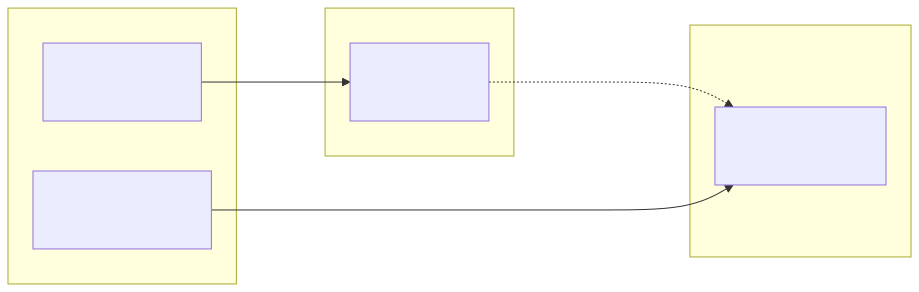
\includegraphics[keepaspectratio,alt={Diagram 11}]{diagrams/tour-11.pdf}}
\caption{Diagram 11}
\end{figure}

\textbf{Structural sharing}: Only changed segments are newly written.
Unchanged data is referenced by hash.

\subsection{7.4 Hash Algorithm Details}\label{hash-algorithm-details}

\textbf{State Root} (BLAKE3, v2):

\begin{verbatim}
state_root = BLAKE3(
    root_id[32]                    ||
    instance_count[8, LE]          ||
    for each instance in BTreeMap order:
        warp_id_len[8, LE]         ||
        warp_id_bytes              ||
        node_count[8, LE]          ||
        for each node in ascending NodeId order:
            node_id[32]            ||
            node_type[32]          ||
            for each outbound edge in ascending EdgeId order:
                edge_id[32]        ||
                edge_type[32]      ||
                to_node[32]        ||
            for each attachment:
                key_len[8, LE]     ||
                key_bytes          ||
                type_id[32]        ||
                value_len[8, LE]   ||
                value_bytes
)
\end{verbatim}

\begin{claudecommentary}
**Claude's Take**: The hashing is *exhaustive*. Every node, every edge, every attachment, every byte—all streamed through BLAKE3 in a defined order. There's no "we'll just hash the IDs and trust the content"—everything participates.

This is expensive! But it's the foundation of Echo's trust model. If two engines produce the same state root, they have the same state. Period. No exceptions, no edge cases.

The `version_tag` in the commit hash is a nice touch. If Echo ever changes its hashing algorithm (say, BLAKE3 v2 to v3), old and new hashes won't collide. Protocol evolution is built in.
\end{claudecommentary}

\begin{center}\rule{0.5\linewidth}{0.5pt}\end{center}

\section{8. Worked Example: Tracing a Link
Click}\label{worked-example-tracing-a-link-click}

Let's trace what happens when a user clicks a link in a hypothetical
WARP-based navigation system.

\subsection{8.1 The Scenario}\label{the-scenario}

Imagine a simple site with two pages:

\begin{figure}
\centering
\pandocbounded{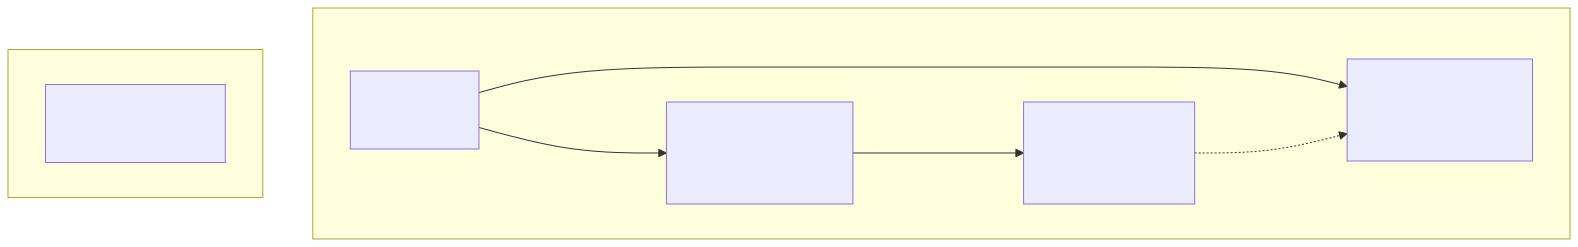
\includegraphics[keepaspectratio,alt={Diagram 12}]{diagrams/tour-12.pdf}}
\caption{Diagram 12}
\end{figure}

\textbf{User clicks the link}: This should navigate from Home to About.

\begin{claudecommentary}
**Claude's Take**: This example is deceptively simple—two pages, one link—but it exercises the entire engine: intent ingestion, rule matching, footprint validation, execution, merge, hashing, and emission.

I'll add my notes at the interesting points. If you're skimming, watch for where the determinism guarantees kick in.
\end{claudecommentary}

\subsection{8.2 Step 1: Intent Ingestion}\label{step-1-intent-ingestion}

The click is captured by the viewer and converted to an \textbf{intent}:

\begin{Shaded}
\begin{Highlighting}[]
\CommentTok{// In the viewer:}
\KeywordTok{let}\NormalTok{ intent }\OperatorTok{=}\NormalTok{ NavigateIntent }\OperatorTok{\{}
\NormalTok{    target\_page}\OperatorTok{:}\NormalTok{ about\_node\_id}\OperatorTok{,}
\NormalTok{    timestamp}\OperatorTok{:}\NormalTok{ deterministic\_tick}\OperatorTok{,}
\OperatorTok{\};}
\KeywordTok{let}\NormalTok{ intent\_bytes }\OperatorTok{=}\NormalTok{ canonical\_encode(}\OperatorTok{\&}\NormalTok{intent)}\OperatorTok{;}

\CommentTok{// Send to engine:}
\NormalTok{engine}\OperatorTok{.}\NormalTok{ingest\_intent(intent\_bytes)}\OperatorTok{;}
\end{Highlighting}
\end{Shaded}

\textbf{What happens inside \texttt{ingest\_intent}}:

\begin{figure}
\centering
\pandocbounded{\includegraphics[keepaspectratio,alt={Diagram 13}]{diagrams/tour-13.pdf}}
\caption{Diagram 13}
\end{figure}

\subsection{8.3 Step 2: Begin
Transaction}\label{step-2-begin-transaction}

\begin{Shaded}
\begin{Highlighting}[]
\KeywordTok{let}\NormalTok{ tx }\OperatorTok{=}\NormalTok{ engine}\OperatorTok{.}\NormalTok{begin()}\OperatorTok{;}  \CommentTok{// tx = TxId(1)}
\end{Highlighting}
\end{Shaded}

\subsection{8.4 Step 3: Dispatch Intent}\label{step-3-dispatch-intent}

\begin{Shaded}
\begin{Highlighting}[]
\NormalTok{engine}\OperatorTok{.}\NormalTok{dispatch\_next\_intent(tx)}\OperatorTok{;}
\end{Highlighting}
\end{Shaded}

\textbf{What happens}:

\begin{figure}
\centering
\pandocbounded{\includegraphics[keepaspectratio,alt={Diagram 14}]{diagrams/tour-14.pdf}}
\caption{Diagram 14}
\end{figure}

\subsection{8.5 Step 4: Rule Matching}\label{step-4-rule-matching}

The \texttt{cmd/navigate} rule matches:

\begin{Shaded}
\begin{Highlighting}[]
\CommentTok{// Matcher: Does this intent want navigation?}
\KeywordTok{fn}\NormalTok{ navigate\_matcher(view}\OperatorTok{:}\NormalTok{ GraphView}\OperatorTok{,}\NormalTok{ scope}\OperatorTok{:} \OperatorTok{\&}\NormalTok{NodeId) }\OperatorTok{{-}\textgreater{}} \DataTypeTok{bool} \OperatorTok{\{}
    \KeywordTok{let}\NormalTok{ intent }\OperatorTok{=}\NormalTok{ view}\OperatorTok{.}\NormalTok{node(scope)}\OperatorTok{?;}
\NormalTok{    intent}\OperatorTok{.}\NormalTok{type\_id }\OperatorTok{==} \StringTok{"navigate\_intent"}
\OperatorTok{\}}

\CommentTok{// Footprint: What will we read/write?}
\KeywordTok{fn}\NormalTok{ navigate\_footprint(view}\OperatorTok{:}\NormalTok{ GraphView}\OperatorTok{,}\NormalTok{ scope}\OperatorTok{:} \OperatorTok{\&}\NormalTok{NodeId) }\OperatorTok{{-}\textgreater{}}\NormalTok{ Footprint }\OperatorTok{\{}
\NormalTok{    Footprint }\OperatorTok{\{}
\NormalTok{        n\_read}\OperatorTok{:} \PreprocessorTok{btreeset!}\NormalTok{[scope}\OperatorTok{.}\NormalTok{clone()}\OperatorTok{,}\NormalTok{ viewer\_node]}\OperatorTok{,}
\NormalTok{        n\_write}\OperatorTok{:} \PreprocessorTok{btreeset!}\NormalTok{[]}\OperatorTok{,}
\NormalTok{        a\_read}\OperatorTok{:} \PreprocessorTok{btreeset!}\NormalTok{[]}\OperatorTok{,}
\NormalTok{        a\_write}\OperatorTok{:} \PreprocessorTok{btreeset!}\NormalTok{[}\PreprocessorTok{AttachmentKey::}\NormalTok{new(viewer\_node}\OperatorTok{,} \StringTok{"current"}\NormalTok{)]}\OperatorTok{,}
        \OperatorTok{..}\KeywordTok{default}\NormalTok{()}
    \OperatorTok{\}}
\OperatorTok{\}}
\end{Highlighting}
\end{Shaded}

\begin{claudecommentary}
**Claude's Take**: Notice the footprint. We declare that we'll:
- **Read** two nodes: the intent (to get the target) and the viewer (to validate the current page)
- **Write** one attachment: the viewer's `current` attachment

We're *not* reading any attachments (we just need the node records), and we're *not* writing any nodes (the viewer node already exists). This precision matters—if another rule also wants to write `viewer.current`, there's a conflict.
\end{claudecommentary}

The rule is enqueued:

\begin{verbatim}
┌─────────────────────────────────────────────────────────────┐
│ PendingRewrite                                               │
├─────────────────────────────────────────────────────────────┤
│ rule_id: "cmd/navigate"                                     │
│ scope: 0xABCD... (intent node)                             │
│ footprint: { n_read: [intent, viewer], a_write: [current] } │
│ tx: TxId(1)                                                 │
└─────────────────────────────────────────────────────────────┘
\end{verbatim}

\subsection{8.6 Step 5: Commit}\label{step-5-commit}

\begin{Shaded}
\begin{Highlighting}[]
\KeywordTok{let}\NormalTok{ (snapshot}\OperatorTok{,}\NormalTok{ receipt}\OperatorTok{,}\NormalTok{ patch) }\OperatorTok{=}\NormalTok{ engine}\OperatorTok{.}\NormalTok{commit\_with\_receipt(tx)}\OperatorTok{;}
\end{Highlighting}
\end{Shaded}

\subsubsection{5a. Drain}\label{a.-drain}

\begin{Shaded}
\begin{Highlighting}[]
\KeywordTok{let}\NormalTok{ rewrites }\OperatorTok{=}\NormalTok{ scheduler}\OperatorTok{.}\NormalTok{drain\_for\_tx(tx)}\OperatorTok{;}
\CommentTok{// Result: [PendingRewrite \{ rule: "cmd/navigate", scope: intent\_node \}]}
\end{Highlighting}
\end{Shaded}

\subsubsection{5b. Reserve}\label{b.-reserve}

\begin{Shaded}
\begin{Highlighting}[]
\CommentTok{// Check footprint independence}
\CommentTok{// No conflicts (only one rewrite)}
\CommentTok{// Accepted!}
\end{Highlighting}
\end{Shaded}

\subsubsection{5c. Execute}\label{c.-execute}

\begin{Shaded}
\begin{Highlighting}[]
\KeywordTok{fn}\NormalTok{ navigate\_executor(view}\OperatorTok{:}\NormalTok{ GraphView}\OperatorTok{,}\NormalTok{ scope}\OperatorTok{:} \OperatorTok{\&}\NormalTok{NodeId}\OperatorTok{,}\NormalTok{ delta}\OperatorTok{:} \OperatorTok{\&}\KeywordTok{mut}\NormalTok{ TickDelta) }\OperatorTok{\{}
    \CommentTok{// Read the intent to find target}
    \KeywordTok{let}\NormalTok{ intent }\OperatorTok{=}\NormalTok{ view}\OperatorTok{.}\NormalTok{node(scope)}\OperatorTok{.}\NormalTok{unwrap()}\OperatorTok{;}
    \KeywordTok{let}\NormalTok{ target\_page }\OperatorTok{=}\NormalTok{ intent}\OperatorTok{.}\NormalTok{attachment(}\StringTok{"target"}\NormalTok{)}\OperatorTok{.}\NormalTok{unwrap()}\OperatorTok{;}

    \CommentTok{// Read current viewer state (for logging/validation)}
    \KeywordTok{let}\NormalTok{ viewer }\OperatorTok{=}\NormalTok{ view}\OperatorTok{.}\NormalTok{node(}\OperatorTok{\&}\NormalTok{VIEWER\_NODE)}\OperatorTok{.}\NormalTok{unwrap()}\OperatorTok{;}
    \KeywordTok{let}\NormalTok{ old\_page }\OperatorTok{=}\NormalTok{ viewer}\OperatorTok{.}\NormalTok{attachment(}\StringTok{"current"}\NormalTok{)}\OperatorTok{;}

    \CommentTok{// Emit the change: update viewer\textquotesingle{}s current page}
\NormalTok{    delta}\OperatorTok{.}\NormalTok{emit(}\PreprocessorTok{WarpOp::}\NormalTok{SetAttachment }\OperatorTok{\{}
\NormalTok{        node}\OperatorTok{:}\NormalTok{ VIEWER\_NODE}\OperatorTok{,}
\NormalTok{        key}\OperatorTok{:} \StringTok{"current"}\OperatorTok{.}\NormalTok{into()}\OperatorTok{,}
\NormalTok{        value}\OperatorTok{:} \PreprocessorTok{AttachmentValue::}\NormalTok{Atom(AtomPayload }\OperatorTok{\{}
\NormalTok{            type\_id}\OperatorTok{:} \StringTok{"node\_ref"}\OperatorTok{.}\NormalTok{into()}\OperatorTok{,}
\NormalTok{            bytes}\OperatorTok{:}\NormalTok{ target\_page}\OperatorTok{.}\NormalTok{to\_bytes()}\OperatorTok{,}
        \OperatorTok{\}}\NormalTok{)}\OperatorTok{,}
    \OperatorTok{\}}\NormalTok{)}\OperatorTok{;}
\OperatorTok{\}}
\end{Highlighting}
\end{Shaded}

\textbf{TickDelta now contains}:

\begin{Shaded}
\begin{Highlighting}[]
\NormalTok{[}
\NormalTok{    (}\PreprocessorTok{WarpOp::}\NormalTok{SetAttachment }\OperatorTok{\{}
\NormalTok{        node}\OperatorTok{:}\NormalTok{ viewer\_node}\OperatorTok{,}
\NormalTok{        key}\OperatorTok{:} \StringTok{"current"}\OperatorTok{,}
\NormalTok{        value}\OperatorTok{:}\NormalTok{ about\_node\_id}
    \OperatorTok{\},}\NormalTok{ OpOrigin }\OperatorTok{\{}\NormalTok{ intent\_id}\OperatorTok{:} \DecValTok{1}\OperatorTok{,}\NormalTok{ rule\_id}\OperatorTok{:} \DecValTok{42}\OperatorTok{,}\NormalTok{ match\_ix}\OperatorTok{:} \DecValTok{0}\OperatorTok{,}\NormalTok{ op\_ix}\OperatorTok{:} \DecValTok{0} \OperatorTok{\}}\NormalTok{)}
\NormalTok{]}
\end{Highlighting}
\end{Shaded}

\subsubsection{5d. Merge}\label{d.-merge}

Only one delta, trivial merge:

\begin{Shaded}
\begin{Highlighting}[]
\KeywordTok{let}\NormalTok{ merged\_ops }\OperatorTok{=} \PreprocessorTok{vec!}\NormalTok{[}
    \PreprocessorTok{WarpOp::}\NormalTok{SetAttachment }\OperatorTok{\{}\NormalTok{ node}\OperatorTok{:}\NormalTok{ viewer\_node}\OperatorTok{,}\NormalTok{ key}\OperatorTok{:} \StringTok{"current"}\OperatorTok{,}\NormalTok{ value}\OperatorTok{:}\NormalTok{ about\_node\_id }\OperatorTok{\}}
\NormalTok{]}\OperatorTok{;}
\end{Highlighting}
\end{Shaded}

\subsubsection{5e. Finalize}\label{e.-finalize}

Apply to state:

\begin{Shaded}
\begin{Highlighting}[]
\NormalTok{state}\OperatorTok{.}\NormalTok{set\_attachment(viewer\_node}\OperatorTok{,} \StringTok{"current"}\OperatorTok{,}\NormalTok{ about\_node\_id)}\OperatorTok{;}
\end{Highlighting}
\end{Shaded}

\subsection{8.7 Step 6: Hash Computation}\label{step-6-hash-computation}

\begin{Shaded}
\begin{Highlighting}[]
\CommentTok{// State root: BLAKE3 of reachable graph}
\KeywordTok{let}\NormalTok{ state\_root }\OperatorTok{=}\NormalTok{ compute\_state\_root(}\OperatorTok{\&}\NormalTok{state)}\OperatorTok{;}  \CommentTok{// 0x7890...}

\CommentTok{// Patch digest: BLAKE3 of merged ops}
\KeywordTok{let}\NormalTok{ patch\_digest }\OperatorTok{=}\NormalTok{ compute\_patch\_digest(}\OperatorTok{\&}\NormalTok{merged\_ops)}\OperatorTok{;}  \CommentTok{// 0xDEF0...}

\CommentTok{// Commit hash}
\KeywordTok{let}\NormalTok{ commit\_hash }\OperatorTok{=}\NormalTok{ BLAKE3(}
\NormalTok{    VERSION\_TAG }\OperatorTok{||}
\NormalTok{    [parent\_hash] }\OperatorTok{||}
\NormalTok{    state\_root }\OperatorTok{||}
\NormalTok{    patch\_digest }\OperatorTok{||}
\NormalTok{    policy\_id}
\NormalTok{)}\OperatorTok{;}  \CommentTok{// 0x1234...}
\end{Highlighting}
\end{Shaded}

\subsection{8.8 Step 7: Emit to Tools}\label{step-7-emit-to-tools}

The engine emits a \texttt{WarpDiff} to the session hub:

\begin{Shaded}
\begin{Highlighting}[]
\NormalTok{WarpDiff }\OperatorTok{\{}
\NormalTok{    from\_epoch}\OperatorTok{:} \DecValTok{0}\OperatorTok{,}
\NormalTok{    to\_epoch}\OperatorTok{:} \DecValTok{1}\OperatorTok{,}
\NormalTok{    ops}\OperatorTok{:} \PreprocessorTok{vec!}\NormalTok{[}
        \PreprocessorTok{WarpOp::}\NormalTok{SetAttachment }\OperatorTok{\{}
\NormalTok{            node}\OperatorTok{:}\NormalTok{ viewer\_node}\OperatorTok{,}
\NormalTok{            key}\OperatorTok{:} \StringTok{"current"}\OperatorTok{,}
\NormalTok{            value}\OperatorTok{:}\NormalTok{ about\_node\_id}
        \OperatorTok{\}}
\NormalTok{    ]}\OperatorTok{,}
\NormalTok{    state\_hash}\OperatorTok{:} \DecValTok{0x7890}\OperatorTok{...,}
\OperatorTok{\}}
\end{Highlighting}
\end{Shaded}

\subsection{8.9 Step 8: Viewer Applies
Diff}\label{step-8-viewer-applies-diff}

The viewer receives the diff and updates its rendering:

\begin{Shaded}
\begin{Highlighting}[]
\ControlFlowTok{for}\NormalTok{ op }\KeywordTok{in}\NormalTok{ diff}\OperatorTok{.}\NormalTok{ops }\OperatorTok{\{}
    \ControlFlowTok{match}\NormalTok{ op }\OperatorTok{\{}
        \PreprocessorTok{WarpOp::}\NormalTok{SetAttachment }\OperatorTok{\{}\NormalTok{ node}\OperatorTok{,}\NormalTok{ key}\OperatorTok{,}\NormalTok{ value }\OperatorTok{\}} \OperatorTok{=\textgreater{}} \OperatorTok{\{}
            \ControlFlowTok{if}\NormalTok{ node }\OperatorTok{==}\NormalTok{ viewer\_node }\OperatorTok{\&\&}\NormalTok{ key }\OperatorTok{==} \StringTok{"current"} \OperatorTok{\{}
                \CommentTok{// Update the displayed page}
                \KeywordTok{self}\OperatorTok{.}\NormalTok{navigate\_to(value}\OperatorTok{.}\NormalTok{as\_node\_ref())}\OperatorTok{;}
            \OperatorTok{\}}
        \OperatorTok{\}}
\NormalTok{        \_ }\OperatorTok{=\textgreater{}} \OperatorTok{\{} \CommentTok{/* other ops */} \OperatorTok{\}}
    \OperatorTok{\}}
\OperatorTok{\}}
\end{Highlighting}
\end{Shaded}

\textbf{Result}: The user sees the About page.

\begin{claudecommentary}
**Claude's Take**: That's a lot of machinery for one link click! But here's what we get for free:

1. **Replay**: Save the intent bytes, replay them later, get the exact same state hash
2. **Verification**: Any other engine given the same inputs produces the same commit hash
3. **Undo**: The previous snapshot is still in history; restoring is a pointer swap
4. **Branching**: Fork the state, try a different navigation, compare outcomes

This is the payoff for all the ceremony. A traditional engine would do `viewer.current = about_page` and call it done. Echo builds a *provable audit trail* around every state change.
\end{claudecommentary}

\begin{center}\rule{0.5\linewidth}{0.5pt}\end{center}

\section{9. The Viewer: Observing Echo}\label{the-viewer-observing-echo}

The \texttt{warp-viewer} crate provides real-time visualization of WARP
graphs. It's built on WGPU for cross-platform GPU rendering.

\subsection{9.1 Architecture}\label{architecture}

\begin{figure}
\centering
\pandocbounded{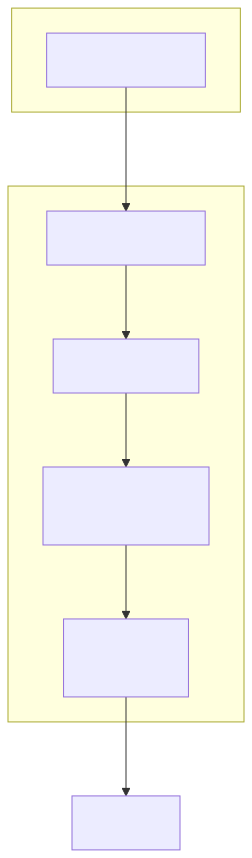
\includegraphics[keepaspectratio,alt={Diagram 15}]{diagrams/tour-15.pdf}}
\caption{Diagram 15}
\end{figure}

\subsection{9.2 Rendering Pipeline}\label{rendering-pipeline}

\begin{enumerate}
\def\labelenumi{\arabic{enumi}.}
\tightlist
\item
  \textbf{Diff arrives} via session client
\item
  \textbf{State cache} updates local graph replica
\item
  \textbf{Layout engine} computes node positions (force-directed)
\item
  \textbf{Renderer} converts graph to GPU buffers
\item
  \textbf{Display} shows updated visualization
\end{enumerate}

\begin{claudecommentary}
**Claude's Take**: The viewer is *reactive*, not poll-based. It subscribes to diffs from the session hub and updates only when state changes. This means zero CPU usage when the graph is idle.

The force-directed layout is a classic choice for graph visualization. It's not perfect—large graphs can take time to settle—but it's good enough for debugging and exploration. If you need a specific layout, you can inject position attachments and the viewer will respect them.
\end{claudecommentary}

\begin{center}\rule{0.5\linewidth}{0.5pt}\end{center}

\section{10. Glossary}\label{glossary}

{\def\LTcaptype{none} % do not increment counter
\begin{longtable}[]{@{}
  >{\raggedright\arraybackslash}p{(\linewidth - 2\tabcolsep) * \real{0.3333}}
  >{\raggedright\arraybackslash}p{(\linewidth - 2\tabcolsep) * \real{0.6667}}@{}}
\toprule\noalign{}
\begin{minipage}[b]{\linewidth}\raggedright
Term
\end{minipage} & \begin{minipage}[b]{\linewidth}\raggedright
Definition
\end{minipage} \\
\midrule\noalign{}
\endhead
\bottomrule\noalign{}
\endlastfoot
\textbf{WARP} & Worldline Algebra for Recursive Provenance---Echo's core
graph model \\
\textbf{Tick} & One complete cycle of the engine (begin → apply → commit
→ hash → record) \\
\textbf{Snapshot} & Immutable point-in-time capture of graph state \\
\textbf{Footprint} & Declaration of resources a rule will read/write \\
\textbf{BOAW} & Bag of Autonomous Workers---parallel execution model \\
\textbf{TickDelta} & Accumulated operations from rule execution \\
\textbf{State Root} & BLAKE3 hash of the entire graph \\
\textbf{Commit Hash} & BLAKE3 hash of (state root + patch + metadata) \\
\textbf{WarpInstance} & A graph-within-a-graph, enabling recursive
composition \\
\textbf{WSC} & Write-Streaming Columnar---Echo's snapshot file format \\
\textbf{GraphView} & Read-only handle to graph state for rule
executors \\
\textbf{PendingRewrite} & Queued rule application awaiting commit \\
\end{longtable}
}

\begin{center}\rule{0.5\linewidth}{0.5pt}\end{center}

\begin{claudecommentary}
**Final Thoughts from Your Tour Guide**

Echo is not a simple system. It's a *principled* system built on hard-won lessons about determinism, reproducibility, and trust.

What I find most impressive isn't any single feature—it's the coherence. Every piece reinforces the others:
- BTreeMaps enable deterministic hashing
- Footprints enable parallel execution
- Parallel execution requires immutable GraphView
- Immutable GraphView enables copy-on-write
- Copy-on-write enables cheap branching
- Cheap branching enables "what if?" queries

Pull one thread and the whole tapestry unravels. This is integrated design, not a collection of independent features.

Is Echo perfect? No. The footprint model requires discipline. The ceremony adds latency. The BTreeMaps trade speed for determinism. But for applications where *provability* matters—games with replays, simulations with audits, collaborative tools with conflict resolution—Echo offers something rare: a foundation you can trust.

Thanks for joining me on this tour. May your state roots always match.

— Claude
\end{claudecommentary}

\backmatter
\end{document}
